\documentclass[final]{jpp}
\usepackage{graphicx}
%\usepackage[utf8]{inputenc}
\usepackage[T1]{fontenc}
\usepackage{amsmath}
\usepackage{amssymb,url,xspace}
\usepackage{bm}
\usepackage{natbib}
\usepackage{float}
\usepackage[colorlinks=true,
  linkcolor=black, citecolor=blue, urlcolor=blue]{hyperref}   % Modify colors of links
\usepackage[dvipsnames,svgnames,x11names,hyperref]{xcolor}  % Load colors for Tikz.
\usepackage[capitalize]{cleveref}
\usepackage{algorithm}    
\usepackage{algpseudocode}  
\usepackage{mathtools}

\usepackage{subcaption}

% plots setup
\usepackage{tikz}                                                               
\usepackage{pgfplots}                                                           
\usepackage{pgfplotstable}                                                      
\usetikzlibrary{patterns}                                   \usepgfplotslibrary{external}                                                   
\pgfplotsset{compat=newest} 
\IfFileExists{./tikzext.perm}{\tikzexternalize[prefix=tikzext/]}{\tikzexternalize}

%------------------------------
% My latex packages
% Author : Baptiste Jimmy Frei
% 2016, EPFL
%-------------------------------
%\NeedsTeXFormat{LaTeX2e}[1994/06/01]
%\ProvidesPackage{mysty}[2016/10/16 My Custom Package]
%
%------------personal command -----------
\newcommand{\grad}{\nabla}
\renewcommand{\vec}[1]{\bm{#1}}

\newcommand{\gradperp}{\nabla_\perp}
\newcommand{\gradpara}{\nabla_\parallel}
\newcommand{\Laplperp}{\nabla^2_\perp}
\newcommand{\Lapl}{\nabla^2}
\renewcommand{\div}{\nabla \cdot}
\newcommand{\rot}{\nabla \times}
\newcommand{\E}{\vec{E}}
\newcommand{\B}{\vec{B}}
\renewcommand{\j}{J}
\renewcommand{\r}{\vec{r}}
\newcommand{\x}{\bm{x}}
\newcommand{\X}{\bm{X}}
\newcommand{\vi}{\bm{v}}
%\newcommand{\p}{\bm{p}}
\newcommand{\q}{\bm{q}}
\newcommand{\dotq}{\dot{\bm q}}
\newcommand{\dotp}{\dot{\bm p}}
\newcommand{\dx}{\bm{\dot{x}}}
\newcommand{\y}{\bm{y}}
\newcommand{\z}{\bm{z}}
\newcommand{\A}{\bm{A}}
\newcommand{\e}{\bm{e}}
\newcommand{\R}{\bm{R}}
\newcommand{\U}{\bm{U}}
\renewcommand{\e}{\bm{e}}
\renewcommand{\k}{\bm k}
\renewcommand{\c}{\bm{c}}
\renewcommand{\a}{\bm{a}}
\newcommand{\vomega}{\vec{\omega}}
\renewcommand{\b}{\vec{b}}
\newcommand{\bgamma}{\bar{\gamma}}
\newcommand{\rhoa}{\bm{\rho}_a}
\newcommand{\gyrhoa}{\overline{\bm{\rho}}_a}

% Fluctuations fields
\newcommand{\dAgc}{\delta \A }
\newcommand{\dApara}{\delta A_\parallel}
\newcommand{\dAgcperp}{\delta \A_{gc,\perp} }
\newcommand{\dAgcpara}{\delta A_{gc,\parallel} }
\newcommand{\dphigc}{\delta \phi}
\newcommand{\dphi}{\delta \phi}
\newcommand{\kperp}{\bm{k}_{\perp}}


% Mathematical operators : 
\newcommand{\px}[1]{\frac{ \partial #1}{\partial x}}
\newcommand{\py}[1]{\frac{ \partial #1}{\partial y}}
\newcommand{\pr}[1]{\frac{ \partial #1}{\partial R}}
\newcommand{\norm}[1]{\left\lVert#1\right\rVert}
\newcommand{\gyaver}[1]{\left<  #1 \right>_{\R}}
\newcommand{\Poissonbracket}[2]{\left\{ #1, #2\right\}}
\newcommand{\pz}[1]{\frac{ \partial #1}{\partial z}}
\newcommand{\corr}[1]{{\color{red}  #1 }}
\newcommand{\dt}[1]{\frac{d #1}{d t}}
\newcommand{\D}{\overline{\mathcal{D}} \circ}      % Differential operator

% Special functions
\newcommand{\bessel}[1]{\mathcal{J}_0\left( #1\right)}
\newcommand{\laguerre}[2]{L_{#1} \left( #2\right)}
\newcommand{\kernel}[1]{\mathcal{K}_{#1}}
\newcommand{\hermite}[2]{H_{#1} \left( #2\right)}

% Guiding-centre operators
\newcommand{\ptheta}{\frac{ \partial }{\partial \theta}}
\newcommand{\ppparallel}{\frac{ \partial }{\partial p_{\parallel}}}
\newcommand{\pmu}{\frac{ \partial }{\partial \mu}}
\newcommand{\pgamma}[1]{\frac{ \partial #1}{\partial \gamma}}
\newcommand{\gammagc}{\overline{\Gamma}_{gc}}
\newcommand{\pvparallel}{\frac{\partial }{ \partial v_{\parallel}}}
\newcommand{\pt}{\frac{\partial}{\partial t}}

% Gyro-centre operators
\newcommand{\gyptheta}{\frac{ \partial }{\partial \overline{\theta}}}
\newcommand{\gyppparallel}{\frac{ \partial }{\partial \overline{p}_{\parallel}}}
\newcommand{\gypvparallel}{\frac{ \partial }{\partial \overline{v}_{\parallel}}}
\newcommand{\gypmu}{\frac{ \partial }{\partial \overline{\mu}}}
\newcommand{\gypgamma}[1]{\frac{ \partial #1}{\partial \overline{\gamma}}}
\newcommand{\gygrad}{\overline{\grad}}
\newcommand{\gammagy}{\overline{\Gamma}_{gy}}
\newcommand{\curvature}{\bm{\kappa}}

% Gyrocentre coordinates 
\newcommand{\gyR}{\overline{\R}}
\newcommand{\gymu}{\overline{\mu}}
\newcommand{\gytheta}{\overline{\theta}}
\newcommand{\gypparallel}{\overline{p}_{\parallel}}
\newcommand{\gyvparallel}{\overline{v}_{\parallel}}
\newcommand{\gyvi}{\overline{\vi}}

% Velocity-space coordinates
\newcommand{\sparallel}{s_{\parallel a}}
\newcommand{\sperp}{s_{\perp a}}
\newcommand{\uparallel}{u_{\parallel a}}
\newcommand{\vparallel}{v_{\parallel}}
\newcommand{\vperp}{v_{\perp}}

% Fluid quantities
\newcommand{\vth}{v_{tha}}
\newcommand{\vthparallel}{v_{th\parallel a }}
\newcommand{\vthperp}{v_{th \perp a}}
\newcommand{\Tperp}{T_{\perp a}}
\newcommand{\Tparallel}{T_{ \parallel a }}
\newcommand{\Pperp}{P_{\perp a}}
\newcommand{\Pparallel}{P_{ \parallel a }}
\newcommand{\Qparallel}{Q_{\parallel  a}}
\newcommand{\Qperp}{Q_{\perp a}}
\newcommand{\gyU}{\overline{\U}}
\newcommand{\gyuparallel}{\overline{u}_{\parallel a}}
\newcommand{\gyvthparallel}{\overline{v}_{th \parallel a}}
\newcommand{\gyTperp}{\overline{T}_{\perp a}}
\newcommand{\gyTparallel}{\overline{T}_{\parallel a}}
% Expansion parameters
\newcommand{\epsilonthperp}{\epsilon_{\perp}^{*}}
\newcommand{\epsilonperp}{\epsilon_\perp}
\newcommand{\epsilonnu}{\epsilon_\nu}

% Set of coordinates
\newcommand{\gccoordinate}{\left( \bm{R}, v_{\parallel}, \mu, \theta, t \right)}
\newcommand{\gccoordinatewphase}{\left( \R, v_{\parallel}, \mu, t \righ)}


% Hermite-Laguerre projector
\newcommand{\momentstar}[2]{ \norm{#2}^{*#1}_a}
\newcommand{\momentall}[2]{ \norm{#2}^{(*)#1}_a}
\newcommand{\moment}[2]{ \norm{#2}^{#1}_a}
\newcommand{\momente}[2]{ \norm{#2}^{#1}_e}
\newcommand{\momentM}[2]{ \norm{#2}^{#1}_{aM}}
\newcommand{\momenta}[1]{\norm{#1}_a}
\newcommand{\momentastar}[1]{\norm{#1}^*_a}
\newcommand{\phaseV}{\mathcal{V}}
\newcommand{\phaseM}{\mathcal{M}}
\newcommand{\momentstare}[2]{ \norm{#2}^{*,#1}_e}
\newcommand{\momentstari}[2]{ \norm{#2}^{*,#1}_i}

% Gyro-center densities
\newcommand{\gyN}{N_a}
\newcommand{\gyNi}{N_i}
\newcommand{\gyNe}{N_e}


% Text-environement marcos
\newcommand{\tZ}{$\mathcal{Z}$ }
\newcommand{\tbZ}{$\bar{\mathcal{Z}}$ }

% math-environement macros
\newcommand{\Z}{\mathcal{Z}}                                % Old phase-space coordinates 
\newcommand{\bZ}{\overline{\mathcal{Z}}}                    % New phase-space coordinates
\newcommand{\Zgc}{\bm{\mathcal{Z}}}                  % Guiding-centre coordinate
\newcommand{\Zgy}{\overline{\bm{\mathcal{Z}}}}       % Gycentre coordinates
\newcommand{\epsilondelta}{\epsilon_{\delta}}               % Amplitude ordering parameter


\newcommand{\T}{\mathcal{T}}         % Coordinate transformation symbol
\newcommand{\Tgc}{\mathcal{T}_{\text{\epsilon,\text{gc}}} }        % Non-perturbative pull-back operator
\newcommand{\Tgy}{\mathcal{T}_{\epsilon,\text{gy}}} % Perturbatibe pull-back operator 

\renewcommand{\L}{\mathcal{L}}       % Lie derivative
\newcommand{\M}{\mathcal{M}}         % Phase-space symbol
\newcommand{\Tpb}{\mathcal{T}^+_\epsilon} % Pull-back operator
\newcommand{\Tpf}{\mathcal{T}^-_\epsilon} % Push-forward operator
\newcommand{\F}{\mathcal{F}}         % Phase-space function w.r.t to old coordinates 
\newcommand{\bF}{\bar{\mathcal{F}} } % Phase-space function w.r.t to new coordinates 
\renewcommand{\L}{\mathcal{L}}         % Lagriangian
\renewcommand{\H}{\mathcal{H}}         % Hamiltonian 
\newcommand{\Hgy}{\overline{\mathcal{H}}_{gy}} % Gyro-centre Hamiltonian

% Distribution function 
% WITHOUT OVERLINE NOTATION
\newcommand{\gyFa}{F_a}   % No overline notation
\newcommand{\overlinegyFa}{\overline{F}_a} 
\newcommand{\overlinegyFaZero}{\overline{F}_{a0}}
\newcommand{\overlinegyFaone}{\overline{F}_{a1}}
\newcommand{\tildegyFa}{\widetilde{F_a}}
\newcommand{\tildegyFao}{\widetilde{F_{a0}}}
\newcommand{\gyFao}{F_{a0}} 
\newcommand{ \gyFaone}{F_{a1}}% Gyrokinetic background
\newcommand{\gyFaM}{F_{aM}} 

\newcommand{\gyFb}{F_b}       % Gyrokinetic b
\newcommand{\gyFe}{F_e} 
\newcommand{\gyFi}{F_i} 
\newcommand{\tildegyFe}{\widetilde{F_e}} 
\newcommand{\tildegyFi}{\widetilde{F_i}}


% WITH OVERLINE
%\newcommand{\tildegyFa}{\widetilde{\overline{F}_a}}
%\newcommand{\tildegyFao}{\widetilde{\overline{F}_{a0}}}
%\newcommand{\gyFao}{\overline{F}_{a0}} 
%\newcommand{ \gyFaone}{\overline{F}_{a1}}% Gyrokinetic background
%\newcommand{\gyFaM}{\overline{F}_{aM}} 

%\newcommand{\gyFb}{\overline{F}_b}       % Gyrokinetic b
%\newcommand{\gyFe}{\overline{F}_e} 
%\newcommand{\gyFi}{\overline{F}_i} 
%\newcommand{\gyFb}{\overline{F}_b}       % Gyrokinetic b
%\newcommand{\tildegyFe}{\widetilde{\overline{F}_e}} 
%\newcommand{\tildegyFi}{\widetilde{\overline{F}_i}}
% Collision operator a 
\newcommand{\gycoll}{\overline{\mathcal{C}}_a}

% Special operator
\newcommand{\kernelcompo}[2]{\left[ #2\right]_{\grad_\perp,#1}}

% Generating function
\newcommand{\G}{\bm{G}}
\newcommand{\GR}{\bm{G}^{\R}}
\newcommand{\Gtheta}{G^{\theta}}
\newcommand{\Gmu}{G^{\mu}}
\newcommand{\Gparallel}{G^{\parallel}}
\newcommand{\ovlgamma}{\overline{\Gamma}}

\newcommand{\dxi}{\text{d} x_I }     % Define linear maps.
\renewcommand{\d}{\text{d}}            % Differential operators

% Some vecotrs notations
\renewcommand{\u}{\vec{u}}
\newcommand{\Fs}{\vec{F}^{[s]}}
\newcommand{\Fns}{\vec{F}^{[ns]}}
\renewcommand{\kperp}{\bm{k}_{\perp}}
\newcommand{\cperp}{\c'_{\perp}}

% Derivative w.r.t shifted velocities
\newcommand{\pwalpha}{\frac{\partial}{\partial w_\alpha}}
\newcommand{\pwbeta}{\frac{\partial}{\partial w_\beta}}
\newcommand{\pwgamma}{\frac{\partial}{\partial w_\gamma}}

\renewcommand{\U}{\bm{U}}
\newcommand{\erf}{\text{erf}}
\newcommand{\w}{\bm{w}}

% Collision command
\newcommand{\gycol}{\overline{C}}

% Some utilities 
\newcommand{\red}[1]{{\color{red}  #1 }}

% Nomenclature cmd shortcut
\newcommand{\nm}[2]{\nomenclature{#1}{#2}}

%--------my include figure------
% new command figure

 %---------------------------------------
    

\DeclarePairedDelimiter\abs{\lvert}{\rvert}
%\DeclarePairedDelimiter\norm{\lVert}{\rVert}


% Format citations
\crefformat{subsection}{\S#1}

\shorttitle{Non-Linear EPW - simulation}
\shortauthor{R. Ancarola}

\title{Numerical simulation and stability study of non-Linear Electron Plasma Waves in a Moment-Based Approach.}

\author{R. Ancarola \aff{1}
  \corresp{\email{raffaele.ancarola@epfl.ch}}}

\affiliation{\aff{1} \'Ecole Polytechnique F\'ed\'erale de Lausanne (EPFL),
  Swiss Plasma Center,
CH-1015 Lausanne, Switzerland}

\begin{document}

\maketitle

\begin{abstract}
This research addresses the numerical simulation of non-linear equations concerning the evolution of electron plasma waves. 
The aim is to study, as a computational engineer,  the implications of using Runge-Kutta methods applied to the first order ODE involved in the system in question.
Most of the report is dedicated to the analysis of the numerical simulation of the equation and, in particular,
a first part concerns the numerical error analysis raised by the finite difference discretization combined by the amplification due to Runge-Kutta explicit schemes. 
Furthermore, a second part studies the equations closure condition in order to reduce unwanted non-physical effects.
\\
More centered on the physics of the problem, the section \ref{sec:dispertion} shows the correctness of the presented non-linear theory in comparison with a reference linear theory (\cite{linear}) in non-collisional regime. At last, a collisionless study on the amplitude of the oscillation is performed in order to show the non-linear uncollisional effects affecting the electron distribution over a long time. 
\end{abstract}

\tableofcontents

\section{Introduction} 

Electron plasma waves is a well-known fundamental phenomena that occur because of the local breaking of the quasineutrality condition in the plasma \cite{thesis5638, Jorge2017}. They occur when the electric field generated by the displacement of electrons in the plasma with respect to a static background of ions. Because of their relative small mass, the electrons are pulled back towards their original position, leading this way to oscillations of the electron plasma density. These oscillations can in turn interact with particles, whose velocity - parallel to the equilibrium magnetic field in a magnetized plasma -is comparable with the phase velocity of the generated waves.
\\
The equation describing this phenomenon - that are the Vlasov and Poisson equations - remains analytically unsolved. However, under particular conditions like high collisionality (allowing for a fluid description), it is possible to predict some related consequences like the non-linear effects of collisions affecting the perturbations (see ref. \cite{thesis5638}). What is done in this research is comparing those results with a numerical simulation and going further in order to study some low collisional phenomena.

\section{Hermite polynomial projection of the drift-kinetic equation}

Starting from the Boltzmann drift-kinetic equation (\cite{Jorge2017}), one can derive a collisional model for the gyroaveraged electron distribution $\gyaver{\gyFe}(t, \R, \vparallel)$,

\begin{equation} \label{eq:drift-kinetic}
\pt \gyaver{\gyFe} + \dot \R\cdot \grad \gyaver{\gyFe} + \dot \vparallel \pvparallel \gyaver{\gyFe} = C_e(\gyaver{\gyFe})
\end{equation}

in the particular case of $\dot \R = v_\parallel \b$, and $\dot \vparallel = e \grad_\parallel \phi/m_e$.
The Lenard-Bernstein collision operator is 
\begin{equation} \label{eq:LenardBernstein}
    C_e = \nu \frac{\partial }{\partial v_\parallel}\left[v_\parallel \gyaver{\gyFe} + \frac{T_e}{m_e} \frac{\partial \gyaver{\gyFe}}{\partial v_\parallel} \right].
\end{equation}
\\
\\
The velocity $\vparallel$ is then decomposed into the drift velocity $u_{\parallel e}$ and the thermal velocity $v_{th \parallel e} = \sqrt{\frac{2 T_{\parallel e}}{m_e}}$, where $T_{\parallel e}$ is the electron temperature. Thus, we define $s_{\parallel e}$ as velocity variable such that 
$\vparallel = u_{\parallel e} + s_{\parallel e} \cdot v_{th \parallel e}(T_{\parallel e})$. 
The aim is to project the electron distribution onto an Hermite polynomial basis w.r.t to the dependence on $\vparallel$, precisely $\gyaver{\gyFe}$ writes:

\begin{equation} \label{eq:projection}
\gyaver{\gyFe} = F_{eM}(\vec{R},\vparallel,t) \sum_{p=0}^{\infty} N_e^p(\R,t) \frac{H_p(s_{\parallel e})}{\sqrt{2^p p!}}
\end{equation}

where $H_p$ (\ref{eq:Hermite}) is the $p^{th}$ degree Hermite polynomial and

\begin{equation}
F_{eM}(\vec{R},\vparallel,t)=\frac{N_e(\vec{R},t)}{v_{th\parallel e}(\vec{R},t)\sqrt{\pi}}\exp\left(-s_{\parallel e}^2\right)    
\end{equation}

The Hermite basis weighted to $\exp(-s_{\parallel e}^2)$ is orthonormal on the $L_2$ integration (\ref{eq:Hermiteorthogonality}), which assures the projection is well defined.
\\
\\
Furthermore, injecting eq. (\ref{eq:projection}) into eq. (\ref{eq:drift-kinetic}) one gets 

\begin{equation} \label{eq:projection-integral}
N_e N_e^p = 2 \pi \int d \mu d \vparallel \frac{B}{m_e} \gyaver{\gyFe} \frac{H_p(s_{\parallel e})}{\sqrt{2^p p!}}.
\end{equation}

Eq. (\ref{eq:drift-kinetic}) is then closed by the poisson equation for the electric potential:

\begin{align} \label{eq:full-poisson}
\grad^2 \phi = 4 \pi e \left( N_{e} - \sum_iN_{i0}\right).
\end{align}

\subsection{Moment hierarchy equations}

Taking now the drift-kinetic equation (\ref{eq:drift-kinetic}) and integrating by the same terms of eq. (\ref{eq:projection-integral}) one gets the following identity:

\begin{equation} \label{eq:projected-drift-kinetic}
    2 \pi \int d \mu d \vparallel \frac{B}{m_e}\frac{H_l(s_{\parallel e})}{\sqrt{2^l l!}} \left[ \pt \gyaver{\gyFe} + v_\parallel \grad_\parallel \gyaver{\gyFe} + \frac{e}{m_e} \grad_\parallel \phi \pvparallel \gyaver{\gyFe} \right] =C_e^l
\end{equation}

where $C_e^l = \int d \vi C_e H_l/(\sqrt{2^ll!})$.
Developing then eq. (\ref{eq:projected-drift-kinetic}),
an equation for the evolution of $N_e$, $T_{\parallel e}$, $u_{\parallel e}$ and each moment $N_e^p$ is derived. The full form is given in the appendix (\ref{eq:moment-hierarchy-appendix}). 
Furthermore, by applying the normalization specified in section (\ref{eq:normalization}) to the full expanded moment hierarchy equation (\ref{eq:moment-hierarchy-appendix}), a final set of equations are obtained (eq. \ref{eq:dlnNdt}, \ref{eq:dlnTdt}, \ref{eq:dudt}, \ref{eq:poisson} and \ref{eq:moment-hierarchy}). Those depend non-linearly on the normalized electron density $\hat{N}$, electron temperature $\hat{T}$, electron parallel velocity $\hat{u}$ and finally the electric field $\hat{\phi}$. 

\begin{align} 
    \frac{\partial \Theta_N}{\partial \hat{t}} =& - \sqrt{2}\hat{u} \frac{\partial \Theta_N}{\partial \hat{z}} - \sqrt{2} \frac{\partial \hat{u}}{\partial \hat{z}} \label{eq:dlnNdt}
    \\
    \frac{\partial\Theta_T}{\partial \hat t} =& 
    -\sqrt{6\hat{T}}N_e^3 \frac{\partial\Theta_N}{\partial \hat{z}}
    -3 \sqrt{\frac{3\hat{T}}{2}} N_e^3 \frac{\partial\Theta_T}{\partial \hat{z}}
    - \hat{u} \frac{\partial\Theta_T}{\partial \hat{z}}
    - 2 \sqrt{2} \frac{\partial \hat{u}}{\partial \hat{z}} 
    - \sqrt{6\hat{T}} \frac{\partial N_e^3}{\partial\hat{z}}
    \label{eq:dlnTdt}
    \\
    \frac{\partial \hat{u}}{\partial \hat t} =& 
    - \hat{\nu} \sqrt{\hat{T}} \hat{u}
    -\frac{\hat{T}}{\sqrt{2}} \frac{\partial \Theta_N}{\partial \hat{z}}
    +\frac{1}{\sqrt{2}}\frac{\partial \hat{\phi}}{\partial \hat{z}}
    -\frac{\hat{T}}{\sqrt{2}} \frac{\partial\Theta_T}{\partial \hat{z}}
    - \sqrt{2} \hat{u} \frac{\partial \hat{u}}{\partial \hat{z}}
    \label{eq:dudt}
    \\
    \frac{\partial^2\hat{\phi}}{\partial \hat{z}^2}=&\hat{N}-1 \label{eq:poisson}
\end{align}

where $\Theta_N = \ln(\hat{N})$ and $\Theta_T = \ln(\hat{T})$.

\begin{align} \label{eq:moment-hierarchy}
\frac{\partial N_e^l}{\partial \hat{t}} =& \sum_p \Omega_p^l N_e^p + \mathcal{I}_p^l \frac{\partial N_e^p}{\partial\hat{z}}  \\
\Omega_p^l :=& \left[ \mathcal{A}^l \hat{\nu} +  \mathcal{B}_p^l \frac{\partial \Theta_N}{\partial \hat{t}} + \mathcal{C}_p^l  \frac{\partial \Theta_N}{\partial \hat{z}}+ \mathcal{D}_p^l \frac{\partial \hat\phi}{\partial \hat{z}}  + \mathcal{E}_p^l \frac{\partial \Theta_T}{\partial \hat{t}} + \mathcal{F}_p^l \frac{\partial \Theta_T}{\partial \hat{z}} \right. \nonumber\\
&\left. + \mathcal{G}_p^l \frac{\partial \hat{u}}{\partial \hat{t}} + \mathcal{H}_p^l  \frac{\partial \hat{u}}{\partial \hat{z}} \right]
\end{align}

with the following coefficients:

\begin{align}
&\mathcal{A}^l = - l \delta_p^l - \sqrt{2l} \hat{u} \delta_p^{l-1} \\
&\mathcal{B}_p^l= -\delta_p^l\\
&\mathcal{C}_p^l=-\left(\sqrt{\hat{T}} \sqrt{l+1}\delta_p^{l+1}+ \sqrt{2}\hat{u} \delta_{p}^{l} +\sqrt{\hat{T}} \sqrt{l}\delta_p^{l-1} \right)\\
&\mathcal{D}_p^l=\sqrt{\frac{l}{\hat{T}}} \delta_p^{l-1} \\
&\mathcal{E}_p^l=- \frac{l}{2}\delta_p^l -\frac{\sqrt{l(l-1)}}{2}\delta_p^{l-2} \\
\end{align}
\begin{align}
&\mathcal{F}_p^l=-\left[\sqrt{\hat{T}} \frac{(l+1)\sqrt{l+1}}{2} \delta_p^{l+1} + \frac{l\hat{u}}{\sqrt{2}} \delta_p^l  +\sqrt{\hat{T}}  l \sqrt{l}\delta_p^{l-1}\right. \nonumber\\
& \left.  \;\;\;\;\;\;\;\;\;\;\;\;\;\;\;\;\;\;+  \hat{u} \frac{\sqrt{l(l-1)}}{2}   \delta_p^{l-2}  + \sqrt{T} \frac{\sqrt{l(l-1)(l-2)}}{2} \delta_p^{l-3} \right] \\
&\mathcal{G}_p^l=- \sqrt{\frac{2l}{\hat{T}}}\delta_p^{l-1} \nonumber\\
&\mathcal{H}_p^l=  - \sqrt{2}(l+1) \delta_p^l - \hat{u}2\sqrt{\frac{l}{\hat{T}}}  \delta_p^{l-1} - \sqrt{2l(l-1)} \delta_p^{l-2} \\
&\mathcal{I}_p^l=-\left(\sqrt{\hat{T}} \sqrt{l+1}\delta_p^{l+1}+\hat{u}\sqrt{2}\delta_p^l + \sqrt{\hat{T}} \sqrt{l}\delta_p^{l-1} \right).
\end{align}

Notice that the form of the moment hierarchy equation (eq. \ref{eq:moment-hierarchy}) is written in a first linear form for fixed $\Theta_N$, $\Theta_T$, $\hat{u}$ and $N_e^3$.
More generally, define the evolving physical quantities vector $\vec{x} = (\vec{\eta}, \vec{N})$, with $\vec{\eta} = \Theta_N, \Theta_T, \hat{u}, N_e^3)$ and $\vec{N} = (N_e^p)_{p \ge 4}$.
The system equations can be then reduced in a first order ODE compact form:

\begin{equation} \label{eq:system}
    \frac{\partial \vec{x}}{\partial \hat{t}}(\hat{t}, \hat{z}) = \vec{G}(\vec{x}(\hat{t}, \hat{z})).
\end{equation}

$G_{\Theta_N}$, $G_{\Theta_T}$ and $G_{\hat{u}}$ depend non-linearly on on $\vec{\eta}$, $G_{N_e^3}$ depends on $\vec{\eta}$ and $N_e^4$ and, finally, $(G_{N_e^p})_{p \ge 4}$ describes a linear system w.r.t. the set of moments $\vec{N}$.

\subsection{Initial conditions}

The poisson equation (\ref{eq:poisson}) and the periodic boundary conditions on $\hat{z}$ imply that the normalized electron density allows the following initial condition:

\begin{equation}
    \Theta_N = \ln(1 + \delta \sin(\hat{k} \hat{z}))
\end{equation}

with $\abs{\delta} < 1$. The temperature $\hat{T}$ is initially set to $1$, then $\Theta_T(\hat{t} = 0) = 0$ , and finally $\hat{u}(\hat{t} = 0) = N_e^p(\hat{t} = 0) = 0$ for all $p \ge 3$. 

\section{Simulation scheme}

The system is numerically simulated on the two degrees of freedom $\hat{z}$ and $\hat{t}$. Thus, for the space description, a one dimensional finite difference discretization is used and the derivative w.r.t to $\hat{z}$ is evaluated as centered at the fourth order (\cite{fdwiki}).  In the special case of $\hat{u}$, the grid is shifted for precision improvement (see \ref{fig:grids}).

\begin{figure}
\centering
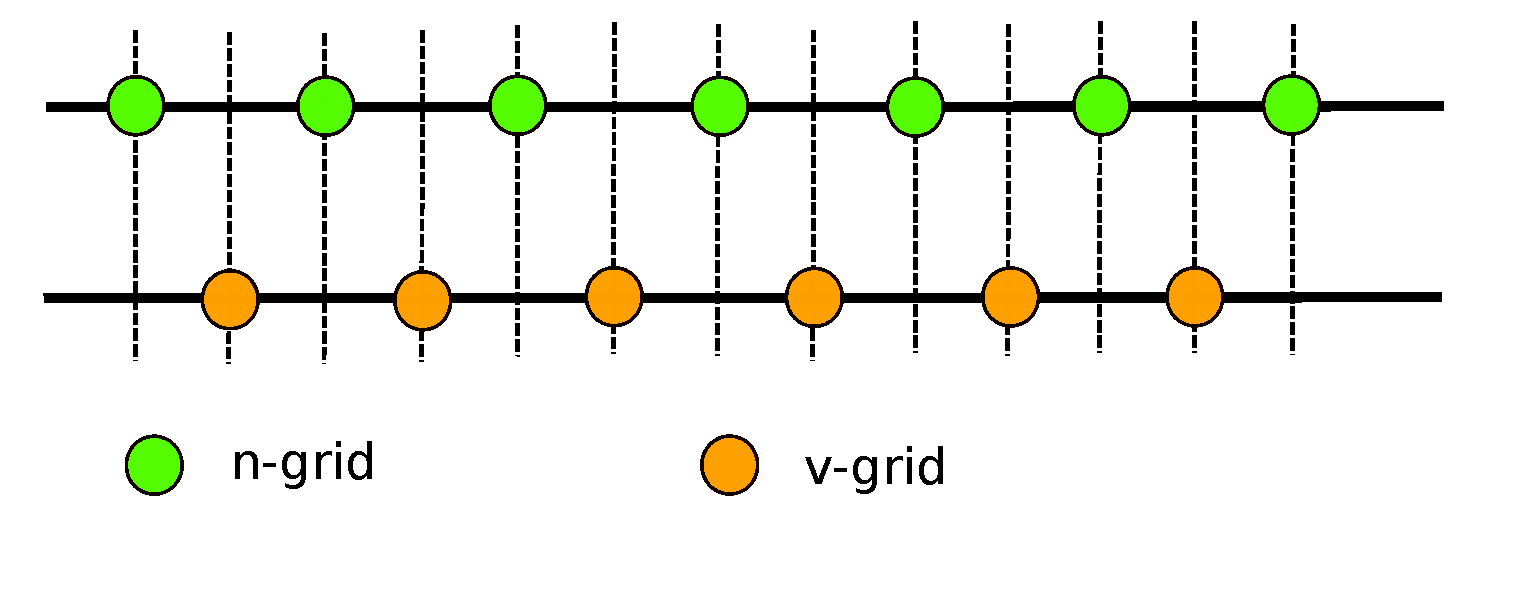
\includegraphics[width=\textwidth]{grid.pdf}
\caption{Representation of the discretization points in \textit{n-grid} and in \textit{v-grid}. \textit{v-grid} is used only for $\hat{u}$, otherwise all other quantities are evaluated on \textit{n-grid}.}
\label{fig:grids}
\end{figure}

The time evolution is performed by different possibilities of Runge-Kutta scheme for the numerical integration of first order ODEs. In particular, it's been used the standard explicit \textit{DOPRI5} (\cite{springer}), the first order runge kutta Chebyshev \textit{RKC4} from \textit{Towards optimal explicit time-stepping schemes for the gyrokinetic equations} of Doerk (\cite{doerk}) and finally the semi-explicit \textit{IMEXRKCB4} from \textit{Low-storage implicit/explicit Runge–Kutta schemes for the
simulation of stiff high-dimensional ODE systems} Cavaglieri (\cite{lowstorageimex}). The butcher tableaux are presented in tables (\ref{tab:rkc4}) and (\ref{tab:imexrkcb4}).

\subsubsection{\textit{IMEXRKCB4} implementation}
The method involves an \textit{ERK} (explicit runge-kutta) and a \textit{DIRK} (diagonally implicit runge-kutta) component. The quantities $\Theta_N$, $\Theta_T$, $\hat{u}$ and the first moment $N_e^3$ are all simulated using a full \textit{ERK}.

\subsubsection{Compromise between numerical stability and performance}
The choice of these methods are motivated by the necessity of stability for the simulation of stiff equations. In particular, the \textit{RKC4} method reveals to be the fastest and \textit{DOPRI5} is nearly comparable, but both are mostly affected by stability issues growing with the number of simulated moments. The \textit{IMEXRKCB4} method, on the other hand, is significantly slower but it allows to simulate an unlimited number of moments.


\begin{table}
\renewcommand\arraystretch{1.2}
\[
\begin{array}
{c|cccc}
0\\
0.03221719644 & 0.03221719644 \\
-1.987635269 & 0 & -1.987635269 \\
0.03221719644 & 0 & 0& 0.03221719644\\
\hline
& 0.001610859822 & 0.11936272179 & -0.2816076282  & 1.160634047 
\end{array}
\]
\caption{RKC4 butcher tableau (\cite{doerk}), stabilized explicit method, order $\mathcal{O}(\Delta t)$.}
\label{tab:rkc4}
\end{table}

\begin{table}
\renewcommand\arraystretch{1.2}
\begin{subtable}{0.5\textwidth}
\[
\begin{array}
{c|cccccc}
0 & 0\\
c_2 & \frac{c_2}{2} & \frac{c_2}{2} \\
c_3 & a_{31}^{IM} & a_{32}^{IM} & a_{33}^{IM} \\
c_4 & b_1 & a_{42}^{IM} & a_{43}^{IM} & a_{44}^{IM} \\
c_5 & b_1 & b_2 & a_{53}^{IM} & a_{54}^{IM} & a_{55}^{IM}\\
1 & b_1 & b_2 & b_3 & b_4 & b_5 & b_6 \\
\hline
& b_1 & b_2 & b_3 & b_4 & b_5 & b_6
\end{array}
\]
\caption{IMRK tableau}
\end{subtable}
\begin{subtable}{0.5\textwidth}
\[
\begin{array}
{c|cccccc}
0 & 0\\
c_2 & c_2 & 0 \\
c_3 & a_{31}^{EX} & a_{32}^{EX} & 0 \\
c_4 & b_1 & a_{42}^{EX} & a_{43}^{EX} & 0 \\
c_5 & b_1 & b_2 & a_{53}^{EX} & a_{54}^{EX} & 0\\
1 & b_1 & b_2 & b_3 & a_{64}^{EX} & a_{65}^{EX} & 0 \\
\hline
& b_1 & b_2 & b_3 & b_4 & b_5 & b_6
\end{array}
\]
\caption{ERK tableau}
\end{subtable}
\caption{IMEXRKCB4 butcher tableau (\cite{lowstorageimex}), semi-explicit method, order $\mathcal{O}(\Delta t^4)$. The respective coefficients are listed in appendix (\ref{sec:imex-butcher}).}
\label{tab:imexrkcb4}
\end{table}

\subsection{Numerical stability analysis}

Define the truncation error $\delta \vec{x}$ as the deviation from the exact solution of the system and consider the following linearization for the derivative error:

\begin{align} \label{eq:trunc}
\frac{\partial\delta\vec{x}}{\partial \hat{t}} =
J \cdot \delta\vec{x} + \mathcal{O}(\norm{\delta\vec{x}}^2)
\end{align}

where $J = \frac{\partial \vec{G}}{\partial\vec{x}}$ is called the \textit{Jacobian} of the system. Although $\vec{G}(\vec{x})$ is an explicit function of $\vec{x}$, we will suppose $J$ as constant because the interest is to study the local behaviour of the truncation error approximating its evolution to a linear decay.

Any \textit{Runge-Kutta} scheme of order $s$ processes the truncation error in the same way as the exact solution, adding the same contributions. More specifically, in the linear approximation:

\begin{align} \label{eq:rktrunc}
\delta\vec{x}_k &= \delta\vec{x}^{(n)} + \sum_{j=1}^{k-1} a_{k,j} \Delta t \vec{J}_k \\
\vec{J}_k &= J \vec{\delta \vec{x}}_k \\
\delta\vec{x}^{(n+1)} &= \delta\vec{x}^{(n)} + \sum_{j=1}^{s} b_j \Delta t \vec{J}_k \label{eq:rktruncstep}
\end{align}

Developing then the recurrence relation of eq. (\ref{eq:rktrunc}), the step \ref{eq:rktruncstep} can be rewritten as follow:

\begin{equation} \label{eq:rktruncpoly}
\delta\vec{x}^{(n+1)} =  (1 + \sum_{j=1}^{s} b_j \Delta t \cdot J) \delta\vec{x}^{(n)} + \sum_{j=1}^{s} \sum_{i=1}{j-1} b_j a_{j,i} (\Delta t \cdot J)^2 \delta\vec{x}_i = \dots =: \sigma(\Delta t \cdot J) \delta\vec{x}^{(n)}
\end{equation}

where $\sigma(z)$ is a polynomial derived from the expansion of eq. \ref{eq:rktruncpoly}. 
Let's say now that $J$ is diagonalizable. Let's call $\{\lambda_i\}_i$ its eigenvalues and $P$ an invertible matrix such that $J = P D P^{-1}$, where $D = diag(\{\lambda_i\})$. 

\begin{equation} \label{eq:rktruncdiag}
\delta\vec{x}^{(n+1)} = P \cdot \sigma(\Delta t \cdot D) \cdot P^{-1} \delta\vec{x}^{(n)}
\end{equation}

The function $\sigma : \mathbb{C} \rightarrow \mathbb{C}$ is called the stability function (see \cite{springer}) because it allows to simply define the domain of absolute stability S as:

\begin{equation} \label{eq:stabdomain}
S = \{z \in \mathbb{C} : \lvert \sigma(z)\rvert \le 1 \}
\end{equation}

If all $z_i = \Delta t \lambda_i \in S$, then the error $\delta \vec{x}$ is exponentially damped for any possible configuration of the system, resulting in a stable behaviour. 
Furthermore, because in a specific time $\hat{t}$ assumes a unique configuration $\vec{x}(\hat{t}, \hat{z})$, then the dominant eigenvalue $\lambda$ makes this condition hold

\begin{equation} \label{eq:eig_current}
J \delta \vec{x} = \lambda \delta \vec{x}.
\end{equation}

\subsubsection{Stability analysis of \textit{RKC4} and \textit{IMEXRKCB4}}
Analysing the absolute stability region of each method, one sees from figure (\ref{fig:rkc4-stability}) that \textit{RKC4} is mostly specialized for a large coverage in the real negative domain, arriving until and extension of $-32$, one order of magnitude higher than the classic Runge-Kutta 4 (\cite{doerk}). \textit{IMEXRKCB4} implicit component (figure \ref{fig:dirk-stability}) is rather unconditionally stable for the whole real negative spectre. The explicit component (figure \ref{fig:erk-stability}) is still comparable to the standard \textit{RK4} method with a small improvement.

\begin{figure}
\begin{subfigure}{0.30 \textwidth}
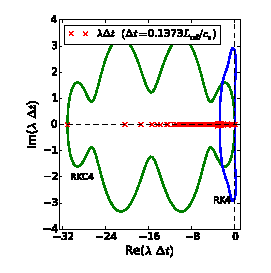
\includegraphics[width=\textwidth]{rkc4-stability.pdf}
\caption{\textit{RKC4} (\cite{doerk}), the curve is compared with the standard \textit{RK4}.}
\label{fig:rkc4-stability}
\end{subfigure}
\hspace{0.02\textwidth}
\begin{subfigure}{0.30 \textwidth}
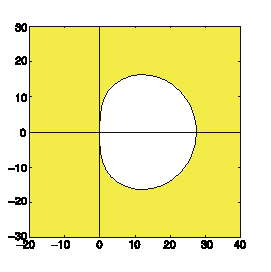
\includegraphics[width=\textwidth]{imex-imrk-stability.pdf}
\caption{\textit{IMEXRKCB4} implicit component (\cite{lowstorageimex})}
\label{fig:dirk-stability}
\end{subfigure}
\hspace{0.02\textwidth}
\begin{subfigure}{0.30 \textwidth}
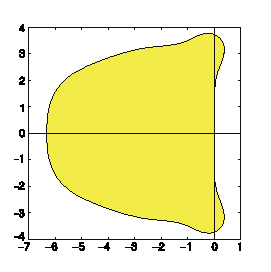
\includegraphics[width=\textwidth]{imex-erk-stability.pdf}
\caption{\textit{IMEXRKCB4} explicit component (\cite{lowstorageimex})}
\label{fig:erk-stability}
\end{subfigure}
\caption{Domain of absolute stability $S$ i.e. values in the complex plane such that $\abs{\sigma} \le 1$.}
\end{figure}

\section{System eigenvalue estimation}

The two schemes \textit{RKC4} and \textit{DOPRI5}, as well as the \textit{ERK} component of \textit{IMEXRKCB4}, are subject to numerical instability due to their small and bounded stability region $S$. Because, given the dominant eigenvalue $\lambda$, the stability condition is $\Delta t \lambda \in S$, it's important to estimate its order of magnitude.

\subsection{Estimation using \texttt{DOPRI5}}

The \textit{DOPRI5} method, as exposed by Ernst Hairer (\cite{springer}), is of high order and its last butcher coefficients are $c_6 = c_7 = 1$. This characteristic allows to define an estimator for the dominant eigenvalue of the jacobian matrix:

\begin{equation} \label{eq:dopri5eig}
\max\abs*{\lambda} := \max_i{\abs*{\lambda_i}} = \frac{\norm{\vec{G}_7 - \vec{G}_6}_V}{\norm{\vec{x}^{(n+1)} - \vec{x}_6}_V}
\end{equation}

for some norm $V$, which can be Hilbert $L_2$ or $\infty$ norm (also called $\max$ norm). The figure (\ref{fig:dopri5eig}) shows that for a test simulation the two norms leads to the same estimation, with more variance in the $\infty$ norm.
Thus, the two estimations are considerable as equivalent and the $L_2$ reveals to be less subject to unwanted oscillations. 
\\
In order to find the dominant term in the moment-hierarchy equation (\ref{eq:moment-hierarchy}) we look at the relation between the dominant eigenvalue and the number of simulated moments. In figure (\ref{fig:dopri5p}) one sees that relation demonstrated by a logarithmic fit showing that $\abs*{\lambda} \propto \sqrt{M}$, where $M$ is the total number of simulated moments.

\begin{figure}
\begin{subfigure}{0.48\textwidth}
\resizebox{\textwidth}{!}{
    \begin{tikzpicture}

\pgfplotsset
{
    %scale only axis,
    %scaled x ticks = base 10:2,
    %height = 18cm,
    width = 9cm,
    xlabel={Number of simulated moments $M$},
    %xmin = 5, xmax = 46,
    legend style = 
    {
        at = {(0.95, 0.1)},
        anchor = south east,
        nodes={scale=1, transform shape}
    },
    %cycle list name = color,
    grid style = dashed,
    ymajorgrids = true,
    minor x tick num = 4,
    %minor y tick num = 4,
    clip mode = individual
}

\pgfplotstableread{dopri5-p.out}\infile

\begin{loglogaxis} 
[
    ylabel={$\max \abs*{\lambda}$},
    log ticks with fixed point
    %ymin = -1.5, ymax = 1.5
]

\addplot
    [
        mark = *,
        color = cyan,
        only marks,
        error bars/.cd,
        y dir=both,
        y explicit
    ]
    table [x = p, y = eig, y error = err] {\infile};
\addlegendentry{Numerical data}

\addplot
    [
        mark = none,
        color = blue,
        domain = 15.0:90.0,
        samples = 50
    ]
    {14.4762 * x^0.54991};
\addlegendentry{$14.47 \cdot M^{0.55 \pm 0.1}$}


\end{loglogaxis}

\end{tikzpicture}

}
\caption{Estimation of the dominant eigenvalue as function of the number of simulated moments.}
\label{fig:dopri5p}
\end{subfigure}
\hspace{0.04\textwidth}
\begin{subfigure}{0.48\textwidth}
\resizebox{\textwidth}{!}{
    \begin{tikzpicture}

\pgfplotsset
{
    %scale only axis,
    %scaled x ticks = base 10:2,
    %height = 18cm,
    width = 9cm,
    xlabel={$\hat{t}$},
    %xmin = 5, xmax = 46,
    legend style = 
    {
        at = {(0.95, 0.70)},
        anchor = north east,
        nodes={scale=1, transform shape}
    },
    %cycle list name = color,
    grid style = dashed,
    ymajorgrids = true,
    minor x tick num = 4,
    %minor y tick num = 4,
    clip mode = individual
}

%\pgfplotstableread{dopri5-estim.out}\infile

\begin{semilogyaxis} 
[
    ylabel={$\max \abs*{\lambda}$},
    %ymin = -1.5, ymax = 1.5
]

\addplot
    [
        mark = asterisk,
        color = red,
        only marks
    ]
    gnuplot [raw gnuplot] {                             plot "dopri5-estim.out" using 1:2;
    };
    %table [x = t, y = l2] {\infile};
\addlegendentry{$\norm{\cdot}_{L_2}$}
    
    
\addplot
    [
        mark = asterisk,
        color = blue,
        only marks
    ]
    gnuplot [raw gnuplot] {                             plot "dopri5-estim.out" using 1:3;
    };
    %table [x = t, y = inf] {\infile};
\addlegendentry{$\norm{\cdot}_{\infty}$}

\end{semilogyaxis}

\end{tikzpicture}

}
\caption{Estimation of the complex module of the dominant eigenvalue of $J$ using \texttt{DOPRI5} method (\ref{eq:dopri5eig}). The test simulation involves $\hat{z} \in [0, 18[$, $\delta = 10^{-2}$, $\hat{\nu} = 0$ and $40$ moments.}
\label{fig:dopri5eig}
\end{subfigure}
\end{figure}

\subsection{Analytical estimation for density, temperature and parallel velocity}

The Jacobian matrix can be analytically derived for the first quantities $\Theta_N$, $\Theta_T$ and $\hat{u}$ from the equations (\ref{eq:dlnNdt}, \ref{eq:dlnTdt}, \ref{eq:dudt}) for a fixed $N_e^3$. 

\begin{minipage}{\textwidth}
\begin{minipage}{0.48\textwidth}
Thus, diagonalizing the obtained matrix it's possible to find the dominant eigenvalue by taking $\lambda \in \mathbb{C}$ such that $\abs{\lambda} = \max\abs{\lambda_i}$. Contrary to the previous analysis, $\lambda$ doesn't correspond to the \textit{global dominant eigenvalue}, but only relatively to the system $(\Theta_N, \Theta_T, \hat{u})$ subject to an external perturbation $N_e^3$.
\\
This analysis allows to study the behaviour of the explicit schemes as function of the initial amplitude $\delta$. In particular, \textit{IMEXRKCB4} stability depends only on this parameter.
\\
In figure (\ref{fig:eig_lambda}) is shown a comparison between the discussed estimations. 
\end{minipage}
\hspace{0.04\textwidth}
\begin{minipage}{0.48\textwidth}
\resizebox{\textwidth}{!}{
    \begin{tikzpicture}

\pgfplotsset
{
    %scale only axis,
    %scaled x ticks = base 10:2,
    %height = 18cm,
    width = 9cm,
    xlabel={$\hat{t}$},
    %xmin = 5, xmax = 46,
    legend style = 
    {
        at = {(0.05, 0.70)},
        anchor = north west,
        nodes={scale=1, transform shape}
    },
    %cycle list name = color,
    grid style = dashed,
    ymajorgrids = true,
    minor x tick num = 4,
    %minor y tick num = 4,
    clip mode = individual
}

%\pgfplotstableread{eig_lambda.out}\infile

\begin{semilogyaxis} 
[
    ylabel={$\max \abs*{\lambda}$},
    %ymin = -1.5, ymax = 1.5
]

\addplot
    [
        mark = asterisk,
        color = orange,
        only marks
    ]
    gnuplot [raw gnuplot] {                             plot "eig_lambda.out" using 1:3;
    };
    %table [x = t, y = ana] {\infile};
\addlegendentry{Analytical}

\addplot
    [
        mark = asterisk,
        color = blue,
        only marks
    ]
    gnuplot [raw gnuplot] {                             plot "eig_lambda.out" using 1:2;
    };
    %table [x = t, y = l2] {\infile};
\addlegendentry{\textit{DOPRI5}}
    
    


\end{semilogyaxis}

\end{tikzpicture}

}
\captionof{figure}{Estimation of the dominant eigenvalue of the subsystem $(\Theta_N, \Theta_T, \hat{u})$. The parameters are $\delta = 10^{-1}$ and $\hat{\nu} = 0$.}
\label{fig:eig_lambda}
\end{minipage}
\vspace{0.5cm}
\end{minipage}

We notice first that the dominant eigenvalue evaluated with the analytical expression upper bounds the eigenvalue estimated with \textit{DOPRI5}. This result means that \textit{DOPRI5} estimates the current leading eigenvalue for the specific error vector $\delta \vec{x}$, equivalently to the relation (\ref{eq:eig_current}). 
\\
Secondly, the analytical estimator gives a purely imaginary eigenvalue with $Im(\lambda) = 18.5 \pm 1.0$. This result means that the motion is mostly advective and, being $\delta = 10^{-1}$ the objective amplitude to be attended, we need to find an optimized $\Delta t$ such that for every scheme we have the stability condition $Im(\Delta t \cdot \lambda) \le 20$. The worst case upper bound of $\abs{\lambda} \le 20$ allows to estimate $\Delta t = 0.15$ for \textit{IMEXRKCB4}, $\Delta t = 0.1$ for \textit{RKC4} and \textit{DOPRI5}.

\subsection{Numerical and temporal limitations}

\subsubsection{RKC4}
The method revealed to be very fast and stable for a large spectrum of values for the collisionality.
In fact the execution time grows linearly in the number of discretization steps and in the number of equations. However for $\hat{\nu} < 10^{-4}$ the method is able to safely simulate until a maximum of 30 moments with $\delta = 10^{-2}$. Because it's full explicit, it's not ideal for long time simulations because many systems, included the concerned one, are always unstable for any $\Delta t$ using explicit schemes.

\subsubsection{IMEXRKCB4}
The round-off error temporally damped independently on the number of simulated equations. However, the growth of execution time is quadratic in the number of discretization steps and equations, consisting in a strong limitation in time complexity. Furthermore, it's ideal for long time simulations with a medium-high number of moments and reasonably small amplitude $\delta$. 

\section{Moments closure condition}

\noindent
\begin{minipage}{\textwidth}
\begin{minipage}{0.45\textwidth}
Similarly as it's shown from \textit{Maria Luisa da Silva Vilelas} in \cite{thesis}, there is a quantity of energy transported through the moments as it's shown in figure (\ref{fig:energy-distribution}). 
The form of the distribution is a cascade where the largest indexed moments carry less energy compared to the first ones $N_e^3$, $N_e^4$, $N_e^5$. From figure (\ref{fig:mom-distrib}) one sees that the phenomenon occurs as well characterized by a constant norm in a first regime for $p \le 130$ and a strong cascade for the highest moments. We call $p_{cut}$ which for $p > p_{cut}$ implies $\norm{N_e^{p+1}}_2 \ll \norm{N_e^p}$.
\end{minipage}
\hspace{0.05\textwidth}
\begin{minipage}{0.48\textwidth}
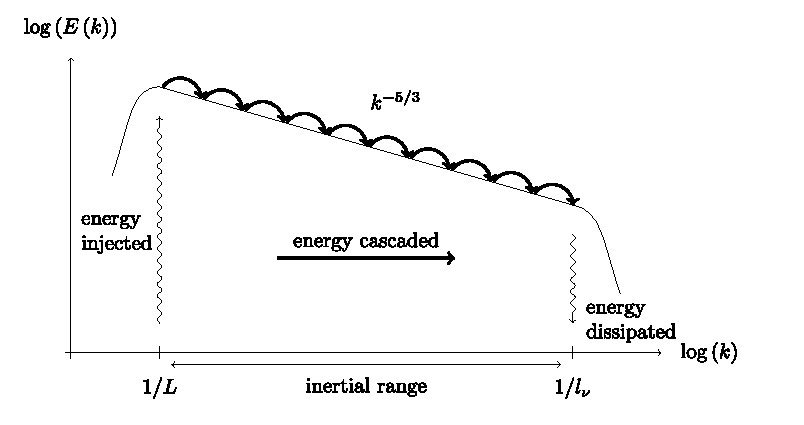
\includegraphics[width=\textwidth]{energy_distribution.pdf}
\captionof{figure}{Distribution of the moments norm in comparison with the energy in paper \cite{thesis}. The higher order moments carry less energy following a curve of diffusion and dissipation.}
\label{fig:energy-distribution}
\end{minipage}
\end{minipage}

\begin{figure}
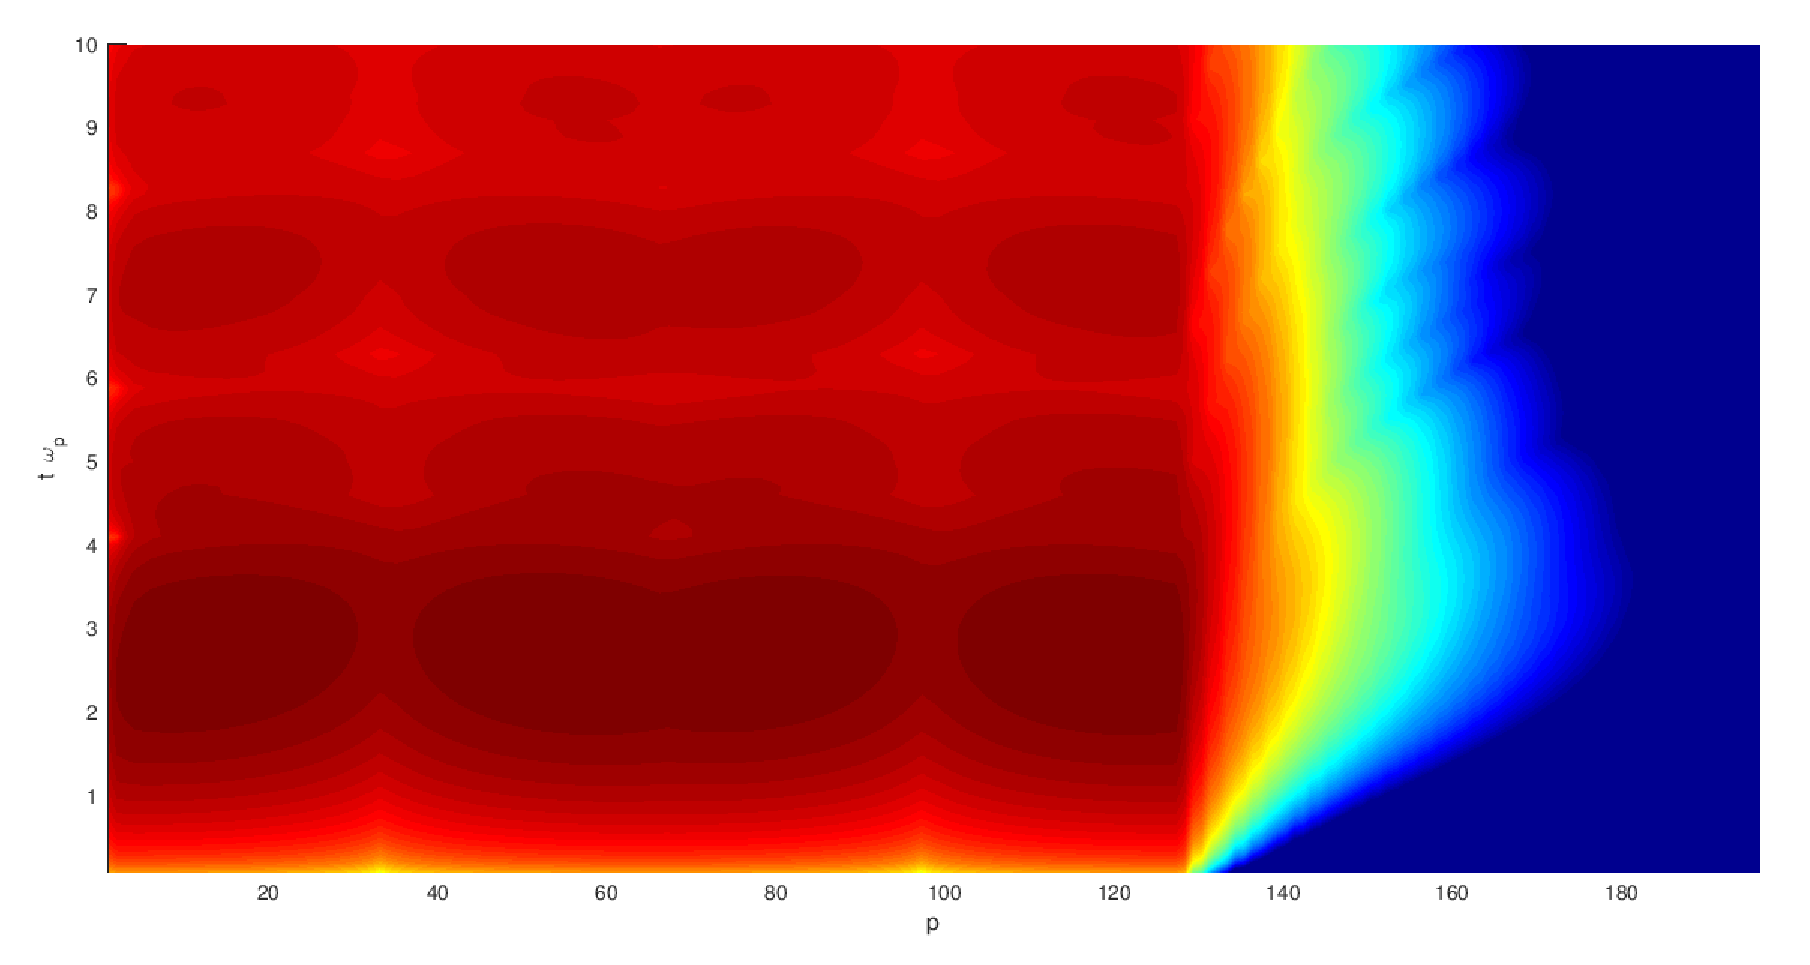
\includegraphics[width=\textwidth]{nu=0.5_mod.eps}
\caption{Distribution of $\norm{N_e^p}_2$ visualized over $M = 200$ moments ($3 \le p \le M$) and $10$ normalized time unit for $\hat{\nu} = 0.5$.}
\label{fig:mom-distrib}
\end{figure}

\subsubsection{Closure numerical effects}
If $M$ is the number of simulated moments, the moment hierarchy equation (\ref{eq:moment-hierarchy}) shows a dependence of the last simulated moment $N_e^M$ on a non-simulated one $N_e^{M+1}$. By a good \textit{closure} is meant an approximated value of $N_e^{M+1}$ emulating a correct resolution of the moment hierarchy equation without perturbations. 

\noindent
\begin{minipage}{\textwidth}
\vspace{0.5cm}
\begin{minipage}{0.4\textwidth}
The simplest closure is found by setting the Dirichlet condition $N_e^{M+1} = 0$.
This closure is really good if $M > p_{cut}$ because the exponential decay of the moment distribution (see figure \ref{fig:collmom}) bounds the amplitude of the moment to infinitely small values, otherwise if $M \le p_{cut}$ the discontinuity gives rise to backwards oscillations. Those are propagating through moment, which lead for long time simulations unwanted non-physical effects.
The bad effect of this closure on the simulated moments can be visualized in figure (\ref{fig:zero-reflection}),
\end{minipage}
\hspace{0.05\textwidth}
\begin{minipage}{0.55\textwidth}
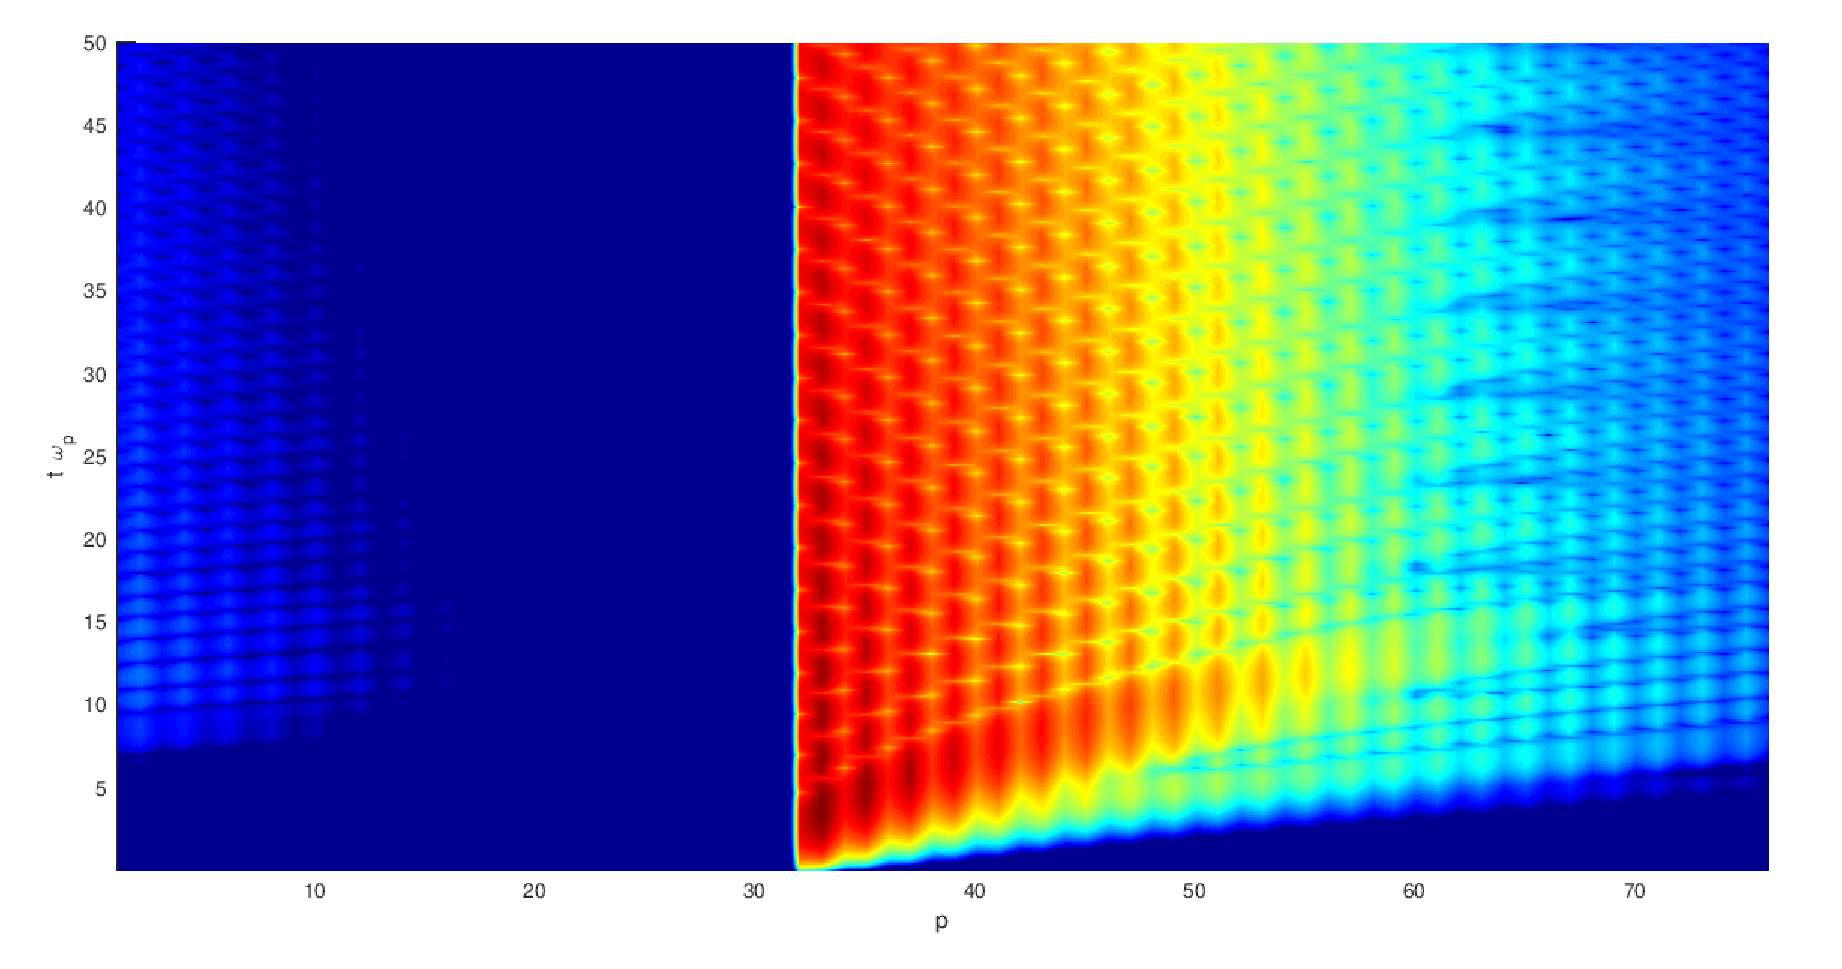
\includegraphics[width=\textwidth]{closure_bounce_mod.eps}
\captionof{figure}{Visualization of $\abs{N_e^p(\hat{z} = 0)}$ with $1 \le p \le 50$. The pattern shows a wave reflecting back from the boundary $p = 50$.}
\label{fig:zero-reflection}
\end{minipage}
\end{minipage}

 where a wave is reflected from the truncation wall $N_e^M$ to the first moments creating a bouncing effect.

\subsection{Dissipation}

This phenomenon is influenced by the collisionality parameter. One sees from figure (\ref{fig:collmom}) and that, for a fixed time point, increasing the collisionality induces a different damping on the distribution curve. Especially there is a point $p_{cut}$, localized around $p = 150$, where the strong damping stops and the curves distinguish themselves depending on the collisionality.

\noindent
\begin{minipage}{\textwidth}
\begin{minipage}{0.47\textwidth}
The purpose is to furnish a prediction for the low collisionality regime and how many moments is necessary to simulate in order to neglect the numerical effects of a zero closure. One sees that overpassed $p_{cut}$, the reflected oscillations of a zero closure are negligible, allowing to calibrate a safe number of moments to simulate. 
\\
On the other hand $p_{cut}$ is a function of time, so there's no warranty that at $\hat{t} = 1$ the distribution will have reached the maximum extension. 
\end{minipage}
\hspace{0.05\textwidth}
\begin{minipage}{0.47\textwidth}
\resizebox{\textwidth}{!}{
    \begin{tikzpicture}

\pgfplotsset
{
    %scale only axis,
    %scaled x ticks = base 10:2,
    %height = 18cm,
    width = 9cm,
    xlabel={$p$},
    %xmin = 5, xmax = 46,
    legend style = 
    {
        at = {(0.05, 0.70)},
        anchor = north west,
        nodes={scale=1, transform shape}
    },
    %cycle list name = color,
    grid style = dashed,
    ymajorgrids = true,
    minor x tick num = 4,
    %minor y tick num = 4,
    clip mode = individual
}

%\pgfplotstableread{collmom.out}\infile

\begin{semilogyaxis} 
[
    ylabel={$\norm{N_e^p}_2 (\hat{t} = 1)$},
    %ymin = -1.5, ymax = 1.5
]

%\addplot+
%    [
%        mark = asterisk,
%        only marks
%    ]
    %table [x = p, y = nu1] {\infile};
%    gnuplot [raw gnuplot] {                             plot "collmom.out" using 1:2;
%    }; 
%\addlegendentry{$\nu = 1$}

\addplot+
    [
        mark = asterisk,
        only marks
    ]
    %table [x = p, y = nu0.5] {\infile};
    gnuplot [raw gnuplot] {                             plot "collmom_new.out" using 1:2;
    };
\addlegendentry{$\nu = 0.5$}

\addplot+
    [
        mark = asterisk,
        only marks
    ]
    %table [x = p, y = nu0.1] {\infile};
    gnuplot [raw gnuplot] {                             plot "collmom_new.out" using 1:3;
    };
\addlegendentry{$\nu = 10^{-1}$}

\addplot+
    [
        mark = asterisk,
        only marks
    ]
    %table [x = p, y = nu0.01] {\infile};
    gnuplot [raw gnuplot] {                             plot "collmom_new.out" using 1:4;
    };
\addlegendentry{$\nu = 10^{-2}$}

\addplot+
    [
        mark = asterisk,
        only marks
    ]
    %table [x = p, y = nu0.001] {\infile};
    gnuplot [raw gnuplot] {                             plot "collmom_new.out" using 1:5;
    };
\addlegendentry{$\nu = 10^{-3}$}

\end{semilogyaxis}

\end{tikzpicture}

}
\captionof{figure}{Moment distribution  $\norm{N_e^p}_2$ for the fixed time $\hat{t} = 1$, $\delta = 0.01$, for different collisionalities.}
\label{fig:collmom}
\end{minipage}
\end{minipage}

\subsection{Polynomial closures}

Considering $N_e^p = N_e(p)$ as a continuous and derivable function over $p > 0$, one can apply a Taylor expansion on $N_e^M$ and choose the order of approximation. Hence,

\begin{equation}
N_e(M + \delta M) = N_e^M + \sum_{i = 1}^\infty \frac{\partial^i N_e}{\partial p^i}|_{p=M} \frac{\delta M^i}{i!}
\end{equation}

With $\delta M = 1$ and approximating the derivative with difference schemes one gets

\begin{align}
N_e^{M+1} &= N_e^M & \text{Order 0} \\
N_e^{M+1} &= 2 N_e^M - N_e^{M-1} & \text{Centred first order} \\
N_e^{M+1} &= 4 N_e^M - 6 N_e^{M-1} + 4 N_e^{M-2} - N_e^{M-3} & \text{Fourth order}
\end{align}

\subsection{Equation derived linear closures}

Although polynomial closures allow to approximate the moments distribution quite well, it often happens that the hypothesis of high order derivability is not applicable. A more suitable approach is deriving a closure specifically basing on the moments hierarchy equation (\ref{eq:moment-hierarchy}).

Considering $l \gg 1$, the amplitude of the  oscillation of $\theta_N$, $\theta_T$, $\hat{u}$ and $N_e^l$ are small enough in order to approximate the moments hierarchy equation in the linear limit. Cutting off all second order terms one gets

\begin{equation} \label{eq:linearmom}
\frac{\partial N_e^l}{\partial \hat{t}} = - \hat{\nu} l N_e^l - \sqrt{\hat{T}} \sqrt{l+1} \frac{\partial N_e^{l+1}}{\partial \hat{z}} - \sqrt{\hat{T}} \sqrt{l} \frac{\partial N_e^{l-1}}{\partial \hat{z}} 
\end{equation}

Considering a statistical steady-state $\frac{\partial}{\partial \hat{t}} = 0$ after the last moment $M+1$ and approximating $N_e^{M+2} \ll N_e^M$, one gets the closure that we call \textit{SSSM} (statistical steady-state moment),

\begin{equation} \label{eq:sssm}
N_e^{M+1} = - \frac{ \sqrt{\hat{T}} }{ \hat{\nu} \sqrt{M+1} } N_e^M 
\end{equation}

Notice that this closure diverges at $\hat{\nu} = 0$. This implies that this closure is consistent only at medium-high collisionality. Furthermore, the observations for the moment distribution (figure \ref{fig:collmom}) is not consistent with the hypothesis for $M < p_{cut}$.

On the other hand, one can derive another relation considering an oscillatory state with small amplitude. Supposing that the normalized plasma frequency $\hat{\omega}$ is known and the damping of the high order moments is mostly collisional, then $N_e^p ~ e^{i(\hat{k}\hat{z} - \hat{\omega}\hat{t}) - \hat{\nu} p t}$. Plugging this relation into eq. \ref{eq:linearmom} one gets a trivial real part and the imaginary lead to the closure that we call \textit{osm} (oscillatory state moment),

\begin{equation}
N_e^{M+1} = \frac{\hat{\omega}}{\sqrt{\hat{T}} \sqrt{M+1}} N_e^M - \sqrt{\frac{M}{M+1}} N_e^{M-1}
\end{equation}

This closure is more consistent for the medium-high order of $M$, because the first term decreases with a factor of $\mathcal{O}(M^{-\frac{1}{2}})$ but it's dominated by a factor $\mathcal{O}(1)$ which explains why the norm $\norm{N_e^p}_2$ is constant for $p < p_{cut}$.
From the results of figure (\ref{fig:collmom}) one deduces that the $L_2$ norm of all moments below $p = 130$ is approximately constant.

\subsection{Effects of the closure in the electric potential}

Numerically, the effect of the closures are mostly visible on the electric potential $\hat{\phi}$ where, interacting with the first moment $N_e^3$, in a certain time produces a bump. The results are shown in figure (\ref{fig:closures}) where one sees that the proposed closures are source of further instability proving the zero closure remains the best for high moments.

\begin{figure}
\centering
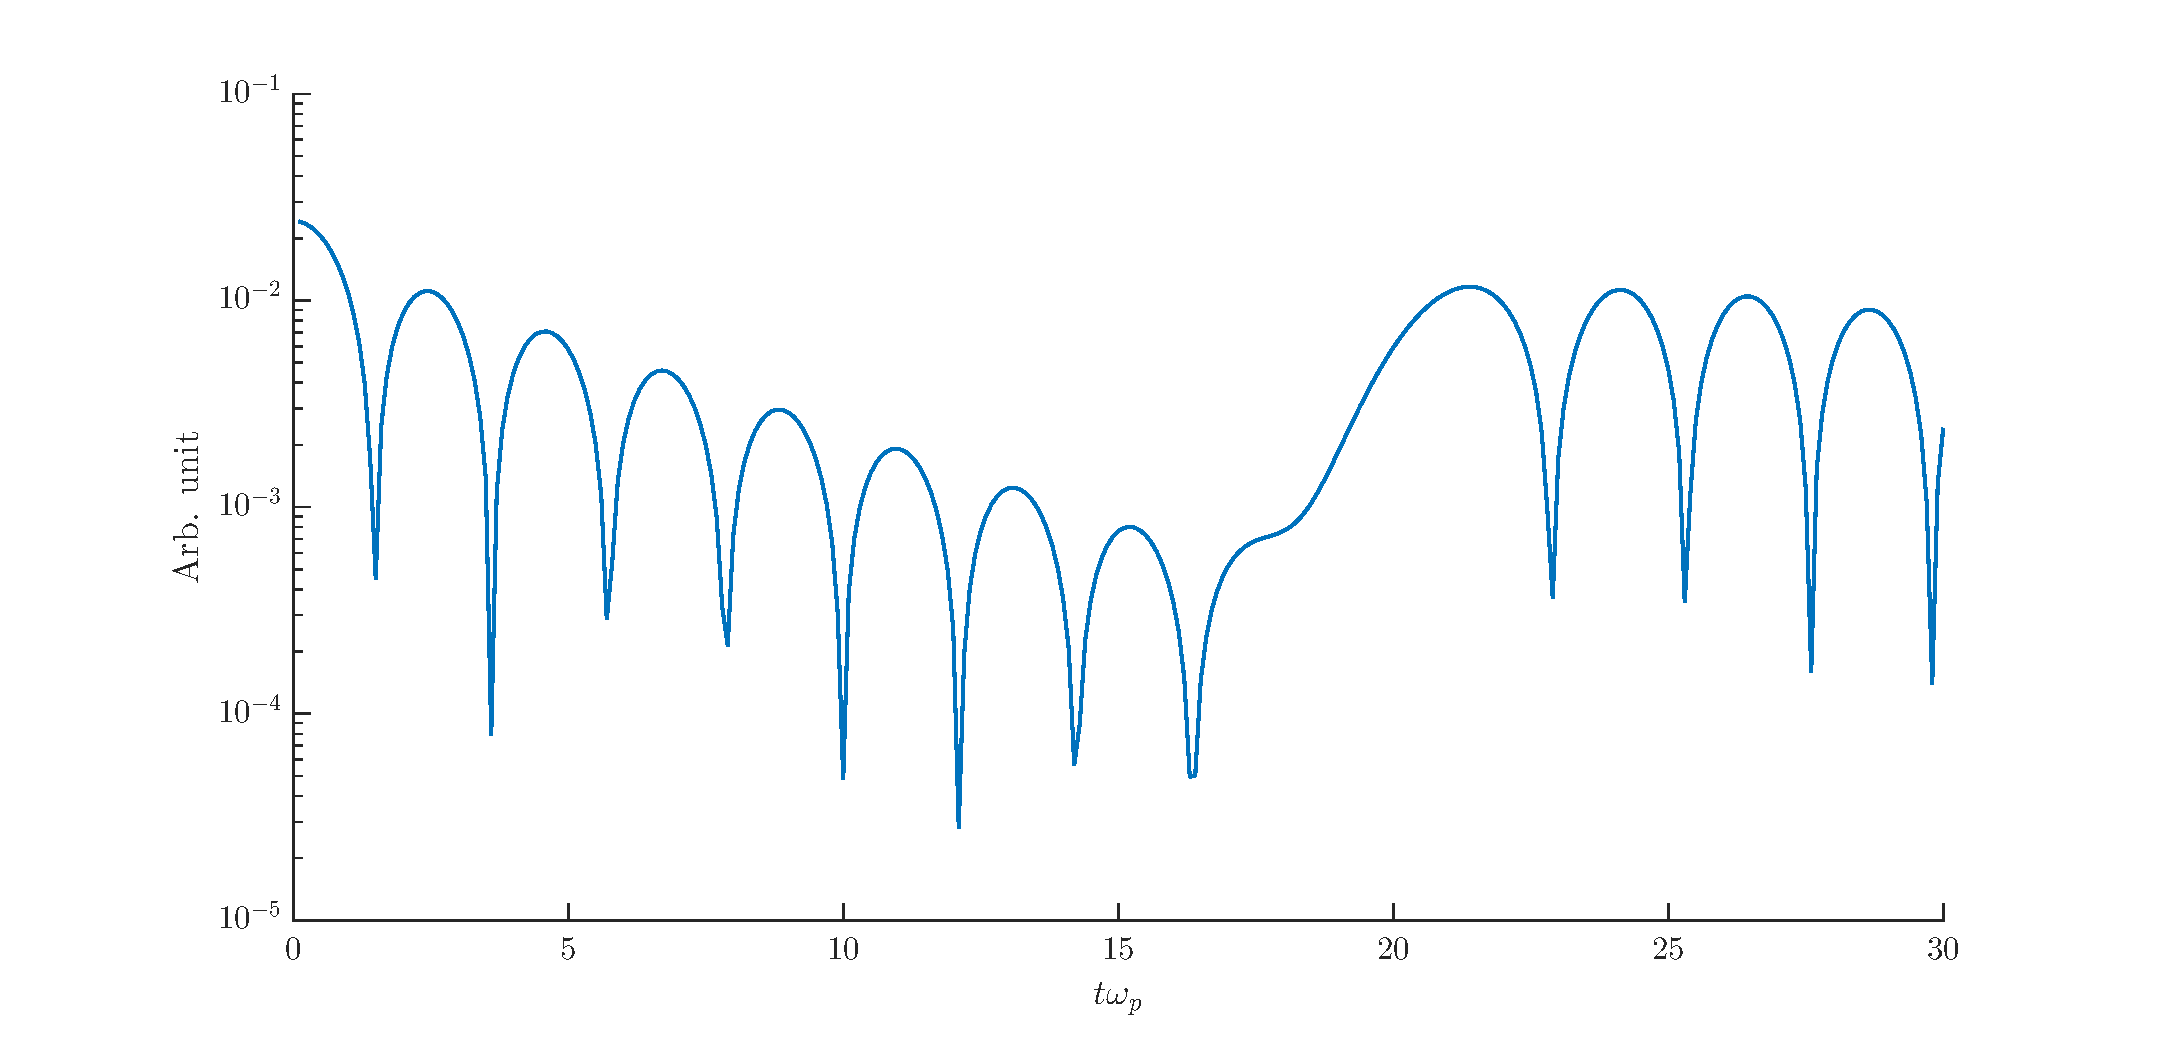
\includegraphics[width=\textwidth]{closure_same.eps}
\caption{Plot of the electric potential norm $\norm{\hat{\phi}}_1$ as function of time for the \textit{osm} closure condition. The bump occurring at time $\hat{t} = 17$ is not a physical effect, but it's due to a discontinuity in the closure condition.}
\label{fig:closures}
\end{figure}

\subsection{Artificial cutoff of the moments}

In order to use the zero closure at the best, one can damp the highest moments artificially in order to cut them off and approximate a solution supposing the highest moments are 

\section{Collisionless dispersion relation} \label{sec:dispertion}

The linear approximation of the drift-kinetic equation predicts an oscillatory regime as analytical solution of the moments (\cite{linear}). In particular, when $\hat{\nu} = 0$ the following dispersion relation holds:

\begin{equation}\label{eq:dispersion}
0 = 1 + \alpha_D - i (\gamma + i\omega)Z(\gamma - i \omega)
\end{equation}
\\
where $Z(x)$ is the plasma dispersion function (\cite{linear}), and $\alpha_D = (2\pi/\hat{z}_{max})^2$, $\gamma$ is the uncollisional damping factor, $\omega$ is the plasma frequency.
The dispersion relation equation is then solved in order to find $\gamma$ and $\omega$.
The same results are expected to be found by applying the current model for $\hat{\nu} = 0$, or rather for $\hat{z}_{max} = 18$, $\gamma = -0.0352$ and $\omega = 1.228$.
\\
The results taken with $\delta = 10^{-3}$ determines a plasma frequency of $\omega = 1.15192$, in accordance with the analytical value obtained by the dispersion relation (\ref{eq:dispersion}) with a relative error of about $6.18\%$.

\begin{figure}
\begin{subfigure}{0.47\textwidth}
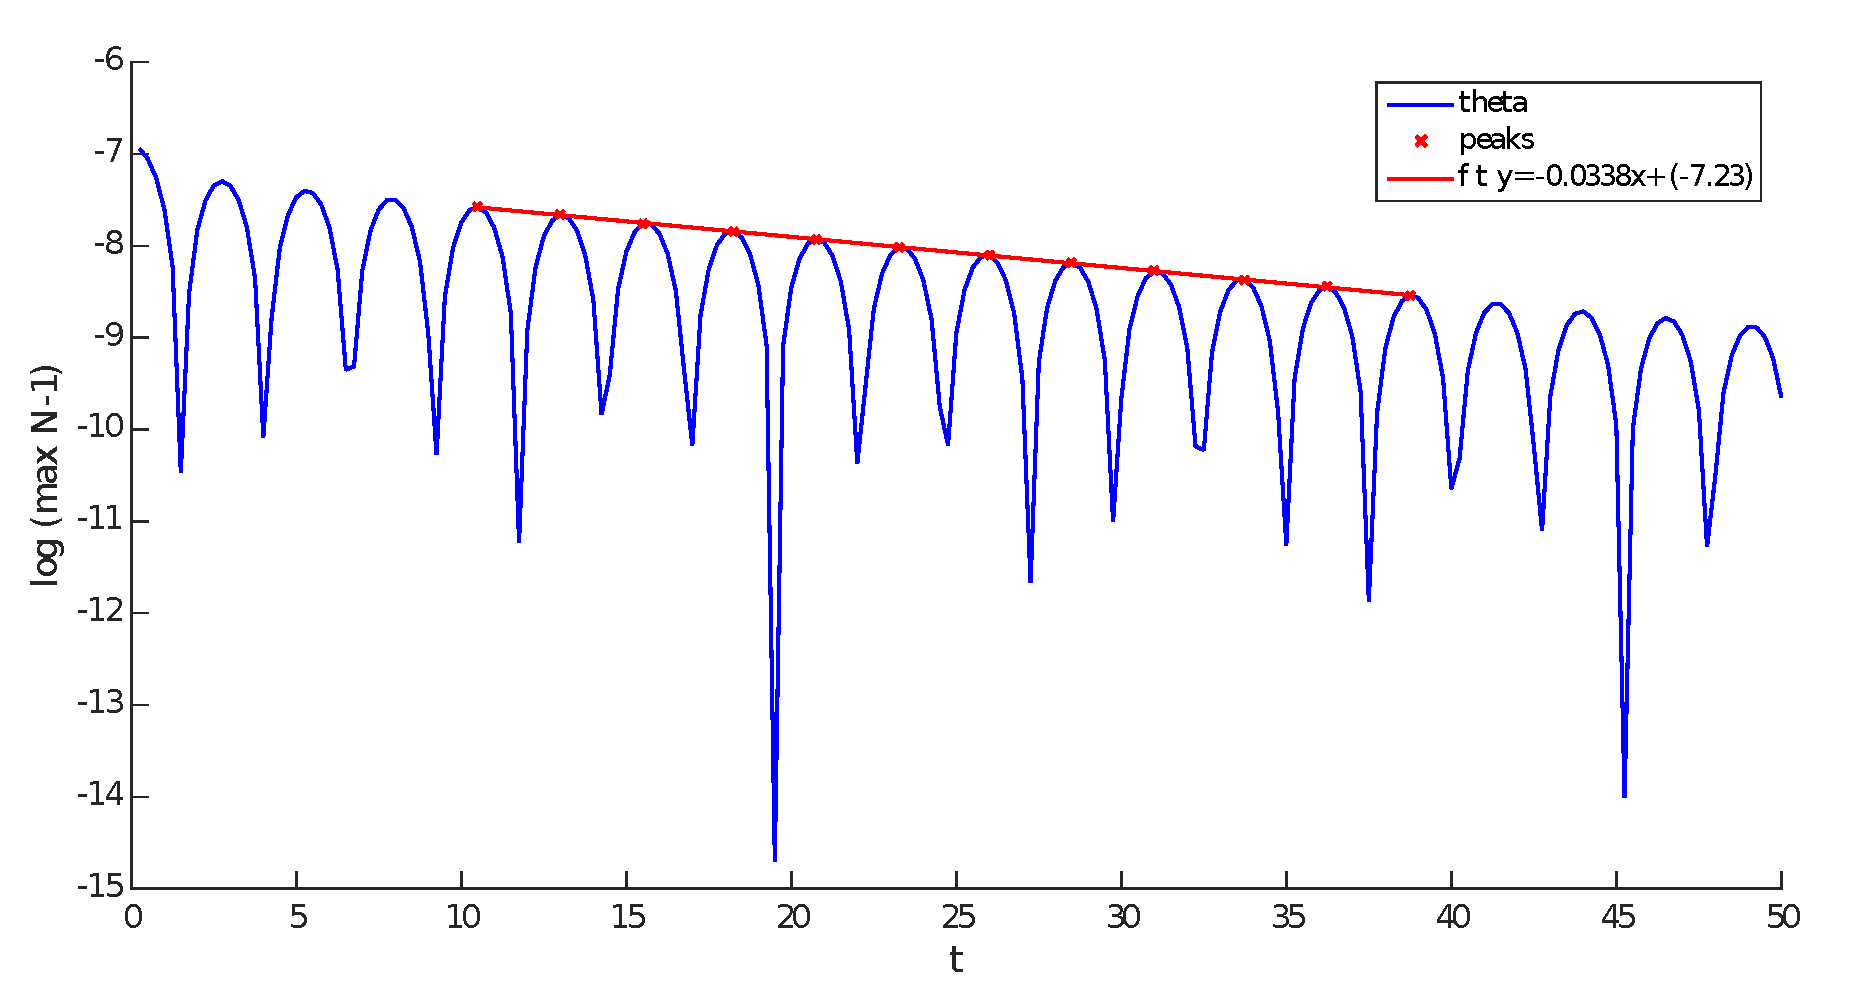
\includegraphics[width=\textwidth]{damping.pdf}
\caption{Logarithmic plot of the amplitude $\max\abs{\hat{N} - 1}$. Uncollisional damping shown for $M = 250$ and $\hat{\nu} = 0$.}
\label{fig:disp-damping}
\end{subfigure}
\hspace{0.05\textwidth}
\begin{subfigure}{0.47\textwidth}
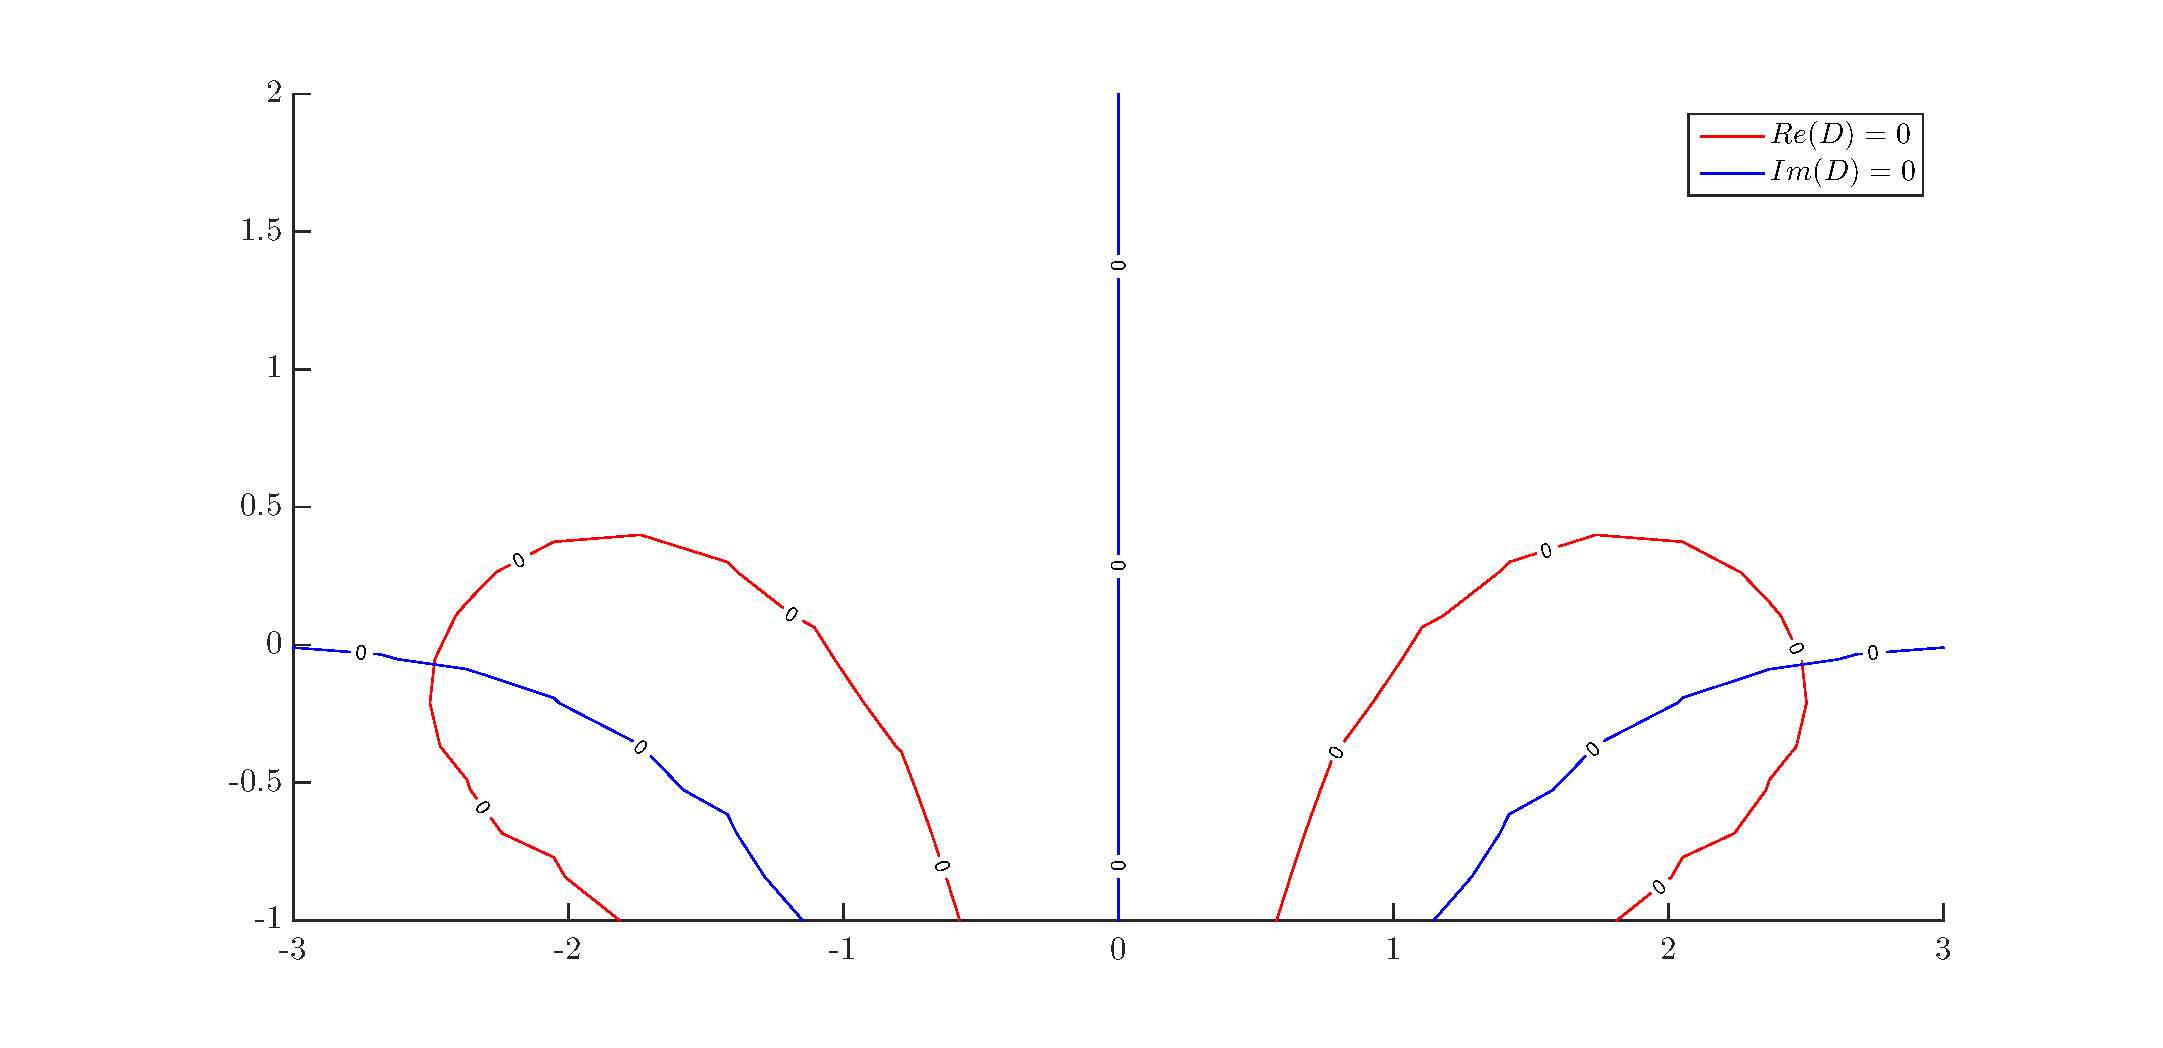
\includegraphics[width=\textwidth]{curve.eps}
\caption{Landau solver: plot of the dispersion relation (\ref{eq:dispersion}). The intersection of the zero curves of the real and the imaginary axis gives the values of $\gamma$ and $\omega$ such that (\ref{eq:dispersion}) is satisfied.}
\label{fig:disp-landau}
\end{subfigure}
\caption{Comparison with the dispertion relation found by the linear theory (\cite{linear}). The damping is influenced by $z_{max} = 18$, implying $\alpha_D = 0.1218$.}
\end{figure}

\begin{figure}
\begin{subfigure}{0.47\textwidth}
\resizebox{\textwidth}{!}{
    \begin{tikzpicture}

\pgfplotsset
{
    %scale only axis,
    %scaled x ticks = base 10:2,
    %height = 18cm,
    width = 9cm,
    xlabel={$\frac{1}{M}$},
    %xmin = 5, xmax = 46,
    legend style = 
    {
        at = {(0.05, 0.50)},
        anchor = north west,
        nodes={scale=1, transform shape}
    },
    %cycle list name = color,
    grid style = dashed,
    ymajorgrids = true,
    minor x tick num = 4,
    %minor y tick num = 4,
    clip mode = individual
}

\pgfplotstableread{dispersion-mom.dat}\infile

\begin{axis} 
[
    ylabel={$\gamma$},
    %ymin = -1.5, ymax = 1.5
]

\addplot
    [
        smooth,
        color = blue,
        mark = *,
        mark options = {
            color = cyan
        }
    ]
    table [x = p, y = damp] {\infile};
    \addlegendentry{$\gamma$ measured}
    %gnuplot [raw gnuplot] {                             plot "dispertion-mom.dat" using 1:2;
    %};
    
\addplot
    [
        color = violet,
        mark = none,
        domain = 0:0.05,
        samples = 10
    ]
    {-0.0351944697912};
    \addlegendentry{$\gamma$ reference}

\end{axis}

\end{tikzpicture}

}
\caption{Number of moments $M$.}
\end{subfigure}
\hspace{0.05\textwidth}
\begin{subfigure}{0.47\textwidth}
\resizebox{\textwidth}{!}{
    \begin{tikzpicture}

\pgfplotsset
{
    %scale only axis,
    %scaled x ticks = base 10:2,
    %height = 18cm,
    width = 9cm,
    xlabel={$\hat{\nu}$},
    %xmin = 5, xmax = 46,
    legend style = 
    {
        at = {(0.05, 0.70)},
        anchor = north west,
        nodes={scale=1, transform shape}
    },
    %cycle list name = color,
    grid style = dashed,
    ymajorgrids = true,
    minor x tick num = 4,
    %minor y tick num = 4,
    clip mode = individual
}

\pgfplotstableread{dispertion-nu.dat}\infile

\begin{semilogxaxis} 
[
    ylabel={$\gamma$},
    %ymin = -1.5, ymax = 1.5
]

\addplot
    [
        smooth,
        mark = asterisk,
        color = red
    ]
    table [x = nu, y = damp] {\infile};
\addlegendentry{$\gamma$ measured}
    
\addplot
[
    color = violet,
    mark = none,
    domain = 0.001:1,
    samples = 10
]
{-0.0351944697912};
\addlegendentry{$\gamma$ reference}

\end{semilogxaxis}

\end{tikzpicture}
}
\caption{Collisionality $\hat{\nu}$.}
\end{subfigure}
\caption{Convergence test of the measured damping $\gamma$ w.r.t the results found by the dispersion relation (\ref{eq:dispersion}) as function of the number of simulated moments $M$ and the collisionality $\hat{\nu}$. The uncollisional limit found by the \textit{Landau} solver is $\gamma = -0.0352$.}
\end{figure}

\section{Non-linear effects}

The linear effects characterizing the moment-hierarchy equation are supposed to produce a equilibrium amplitude of the oscillations for $\hat{t} \to \infty$. After the initial state, where the amplitude damps even without collisionality as it's shown in figure (\ref{fig:disp-damping}), there is a second regime of stationary amplitude due to the dominance of the non-linear effect. In fact, the persistence of \textit{BGK} waves (\cite{thesis5638}) gives raise to a stabilization, which puts the electron electric field in an stable oscillatory regime. In the point of view of the moments, each one synchronized with the other moments reaching an oscillatory limit.  
Studying the value of $\norm{\hat{\phi}}_1$, notice it starts from the one imposed by the initial conditions, or rather

\begin{equation}
\norm{\hat{\phi}}_1 = \frac{2\delta z_{max}}{\phi \alpha_D} 
\end{equation}

and then it damps until converging to a stable value. Unfortunately there's no analytical prediction for that convergence. However we found that there is a clear dependence on the initial amplitude $\delta$.
As it's shown in figure (\ref{fig:long-time}), $\norm{\hat{\phi}}_1$ stops damping in a shorter time if $\delta$ is larger.

\begin{figure}
\resizebox{\textwidth}{!}{
    \begin{tikzpicture}

\pgfplotsset
{
    %scale only axis,
    %scaled x ticks = base 10:2,
    %height = 18cm,
    width = 9cm,
    xlabel={$\hat{t}$},
    %xmin = 5, xmax = 46,
    legend style = 
    {
        at = {(0.95, 0.70)},
        anchor = north east,
        nodes={scale=1, transform shape}
    },
    %cycle list name = color,
    grid style = dashed,
    ymajorgrids = true,
    minor x tick num = 4,
    %minor y tick num = 4,
    clip mode = individual
}

%\pgfplotstableread{dopri5-estim.out}\infile

\begin{semilogyaxis} 
[
    ylabel={$\norm{\hat{\phi}}_1$},
    %ymin = -1.5, ymax = 1.5
]

\addplot
    [
        mark = none,
        color = orange
    ]
    gnuplot [raw gnuplot] {                             plot "plot_phi.dat" using 1:4;
    };
    %table [x = t, y = l2] {\infile};
\addlegendentry{$\delta = 10^{-1}$}

\addplot
    [
        mark = none,
        color = blue
    ]
    gnuplot [raw gnuplot] {                             plot "plot_phi.dat" using 1:3;
    };
    %table [x = t, y = l2] {\infile};
\addlegendentry{$\delta = 10^{-2}$}

\addplot
    [
        mark = none,
        color = red
    ]
    gnuplot [raw gnuplot] {                             plot "plot_phi.dat" using 1:2;
    };
    %table [x = t, y = l2] {\infile};
\addlegendentry{$\delta = 10^{-3}$}
    

\end{semilogyaxis}

\end{tikzpicture}

}
\caption{Plot of $\norm{\hat{\phi}}_1$ until $\hat{t} = 200$ for different initial amplitudes $\delta$. The chosen parameters are $\alpha_D = 0.3$.}
\label{fig:long-time}
\end{figure}

This results is coherent compared with the paper \cite{thesis5638}, where it's shown a similar behaviour. In conclusion, even without collisionality, the electron plasma waves tend to naturally damp until an equilibrium state is reached.

\section{Conclusion}

The moment-based approach applied to the finite difference discretization satisfies the expectations and allows to observe the physical processes in reasonable stability limits. However, there are still some non negligible numerical issues concerning closure and time integration that need further attention in the future.
\\
After the stability analysis and the comparison between the difference Runge-Kutta methods \textit{RKC4} and \textit{IMEXRKCB4}, the main limitations remain the number of simulated moments in terms of execution time and the amplitude $\delta$ in terms of stability. \textit{IMEXRKCB4} requires solving a sparse $\mathcal{O}(n_z \cdot M)$ matrix, which scales in $\mathcal{O}((n_z \cdot M)^2)$ in the solving time complexity in opposition with \textit{RKC4} which requires only $\mathcal{O}(n_z \cdot M)$ of operations per step. On the other hand \textit{IMEXRKCB4} is safer in terms of stability for a large number of simulated moments and often long time simulations require such a method in order to bound the round-off error.
The \textit{RKC4} method is very versatile and also stable enough in order to get good results until 150 simulated moments for medium collisionality ($\nu = 0.1$). Furthermore, it behaves also well for low collisionality simulations allowing to safely reach $\hat{t} = 100$ for $M = 40$.     
\\
Unfortunately, the study on the closure didn't give enough satisfactory results, or rather the best closure still remains the Dirichlet zero condition, which revealed to be valid for a high number of simulated moments. It's been then more important to simulate with $M > p_{cut} = 130$ in order to get reliable results, which has clearly been possible with a greater computational cost. 
\\
In conclusion, the time integration methods proved to be enough reliable for the purpose of this research. 

\section{Appendix}

\subsection{Normalization} \label{sec:norm}

\begin{align} \label{eq:normalization}
 \hat{N}=\frac{N_e}{N_{e0}} & &
 \hat{t}=t \omega_{pe0} &  &  \omega_{pe0}^2=\frac{4\pi N_{e0}e^2}{m_e} \\
 %
\hat{T}=\frac{T_{\parallel e}}{T_{\parallel e0}} & & \hat{\R}=\frac{\R}{\lambda_{De0}} & & \lambda_{De0}^2=\frac{T_{\parallel e0}}{4\pi N_{e0}e^2} \\
%
\hat{u}=\frac{u_{\parallel e}}{v_{th \parallel e}} & &  v_{th \parallel e 0 }= \sqrt{\frac{2 T_{\parallel e0}}{m_e}} =  \lambda_{De0}\omega_{pe0}\sqrt{2 } & &
\end{align}

\subsection{Hermite polynomials} \label{sec:hermite}

\begin{equation} \label{eq:Hermite}
    H_p(x) = (-1)^p e^{x^2} \frac{d^p}{dx^p} e^{-x^2}
\end{equation}

Orthogonality relation:

\begin{equation} \label{eq:Hermiteorthogonality}
    \int_{-\infty}^\infty d x H_l(x) H_{l'}(x) e^{-x^2} = 2^l l! \sqrt{\pi} \delta^l_{l'}
\end{equation}



\subsection{Expanded moment hierarchy equation}

\begin{align}
2 \pi &\int d \mu d \vparallel \frac{B}{m_e}\frac{H_l(s_{\parallel e})}{\sqrt{2^l l!}} \pt \gyaver{\gyFe}  \nonumber \\
=&\pt[\gyNe N_e^l]
+ \frac{\sqrt{2l}}{v_{th \parallel e}}  N_e N_e^{l-1} \frac{\partial u_{\parallel e}}{\partial t}
+ \frac{\partial (\ln T_{\parallel e})}{\partial t}  N_e \left[ \frac{l}{2}N_e^l+ \frac{\sqrt{l(l-1)}}{2}N_e^{l-2} \right],
\end{align}

leading to

\begin{align} \label{eq:moment-hierarchy-appendix}
 &\pt[\gyNe N_e^l] \nonumber\\
 &+\frac{\partial}{\partial z}\left[ u_{\parallel e}N_eN_e^l +  v_{th\parallel e} N_e\left(\sqrt{\frac{l+1}{2}} N_e^{l+1}+ \sqrt{\frac{l}{2}} N_e^{l-1}  \right) \right] \nonumber\\
&- \frac{e}{m_e} \frac{\partial \phi}{\partial z} \frac{\sqrt{2l}}{v_{th\parallel e}} N_e N_e^{l-1}\nonumber\\
&+ \frac{\partial (\ln T_{\parallel e} )}{\partial t} N_e \left[ \frac{l}{2}N_e^l+ \frac{\sqrt{l(l-1)}}{2}  N_e^{l-2} \right] \nonumber\\
&+ v_{th\parallel e} \frac{\partial(\ln T_{\parallel e})}{\partial z}N_e \left[  \frac{l}{2}\sqrt{\frac{l+1}{2}} N_e^{l+1}+\frac{l(2l-1)}{2\sqrt{2l}} N_e^{l-1} + \frac{\sqrt{l(l-1)(l-2)}}{2\sqrt{2}} N_e^{l-3}  \right] \nonumber \\
&+ u_{\parallel e} \frac{\partial (\ln T_{\parallel e})}{\partial z} N_e\left[ \frac{l}{2}N_e^l+ \frac{\sqrt{l(l-1)}}{2}N_e^{l-2} \right] \nonumber\\
& + \frac{\sqrt{2l}}{v_{th \parallel e}}  N_e N_e^{l-1} \frac{\partial u_{\parallel e}}{\partial t} + N_e\left( lN_e^l +\sqrt{l(l-1)}N_e^{l-2}+  \frac{\sqrt{2l} u_{\parallel e}}{v_{th\parallel e}} N_e^{l-1} \right) \frac{\partial u_{\parallel e}}{\partial z} \nonumber\\
&= C_e^l 
\end{align}

\subsection{IMEXRKCB4 butcher coefficients} \label{sec:imex-butcher}

\begin{align*}
&c_2 = \frac{1}{4}, \quad c_3 = \frac{3}{4}, \quad c_4 = \frac{3}{8}, \quad c_5 = \frac{1}{2} \\ 
&b_1 = \frac{232 049 084 587}{1 377 130 630 063} \quad b_2 = \frac{322 009 889 509}{2 243 393 849 156} \quad b_3 = -\frac{195 109 672 787}{1 233 165 545 817} \\
&b_4 = -\frac{340 582 416 761}{705 418 832 319} \quad
b_5 = \frac{463 396 075 661}{409 972 144 477} \quad
b_6 = \frac{323 177 943 294}{1 626 646 580 633} \\
&a_{31}^{IM} = \frac{216 145 252 607}{961 230 882 893} \quad
a_{32}^{IM} = \frac{257 479 850 128}{1 143 310 606 989} \quad
a_{33}^{IM} = \frac{30 481 561 667}{101 628 412 017} \\
&a_{42}^{IM} = -\frac{381 180 097 479}{1 276 440 792 700} \quad
a_{43}^{IM} = - \frac{54 660 926 949}{461 115 766 612} \quad
a_{44}^{IM} = \frac{344 309 628 413}{552 073 727 558} \\
&a_{53}^{IM} = -\frac{100 836 174 740}{861 952 129 159} \quad
a_{54}^{IM} = -\frac{250 423 827 953}{1 283 875 864 443} \quad
a_{55}^{IM} = \frac{1}{2} \\
&a_{31}^{EX} = \frac{153 985 248 130}{1 004 999 853 329} \quad
a_{32}^{EX} = \frac{902 825 336 800}{1 512 825 644 809} \\
&a_{42}^{EX} = \frac{99 316 866 929}{820 744 730 663} \quad
a_{43}^{EX} = \frac{82 888 780 751}{969 573 940 619} \\
&a_{53}^{EX} = \frac{57 501 241 309}{765 040 883 867} \quad
a_{54}^{EX} = \frac{76 345 938 311}{676 824 576 433} \\
&a_{64}^{EX} = - \frac{4 099 309 936 455}{6 310 162 971 841} \quad
a_{65}^{EX} = \frac{1 395 992 540 491}{933 264 948 679}
\end{align*}

\newpage

\bibliographystyle{jpp}
\bibliography{references}

\end{document}